% !TEX root = ../main-es.tex
%TC:macro \limite [ignore,ignore]
%TC:macro \nota [ignore]
%TC:macro \TODO [ignore]
%TC:macro \parencite [ignore]
%TC:macro \textcite [ignore]
\section{Resultados}\label{sec:resultados}

Todas las cifras de esta sección son utilidad neta media sobre 30 semillas, con $p=0.9$, $r=3$ y $c=5$ salvo que se diga otra cosa, y las diferencias entre políticas son pareadas por semilla y se reportan como media $\pm$ EE de la diferencia. En los cuadros, las diferencias en negrita superan dos errores estándar. Las cifras salen de los barridos corridos con la regla de costo corregida (§\ref{sec:regla-costo}).

\subsection{La frontera de fase}\label{sec:res-frontera}

La figura~\ref{fig:frontera} es la figura central del trabajo, pues muestra la utilidad neta contra el dinamismo $\lambda$, con una línea por política y un panel por costo de edición $c$, y el cuadro~\ref{tab:frontera} pone en números las dos comparaciones que la deciden.

\begin{figure}[htbp]
  \centering
  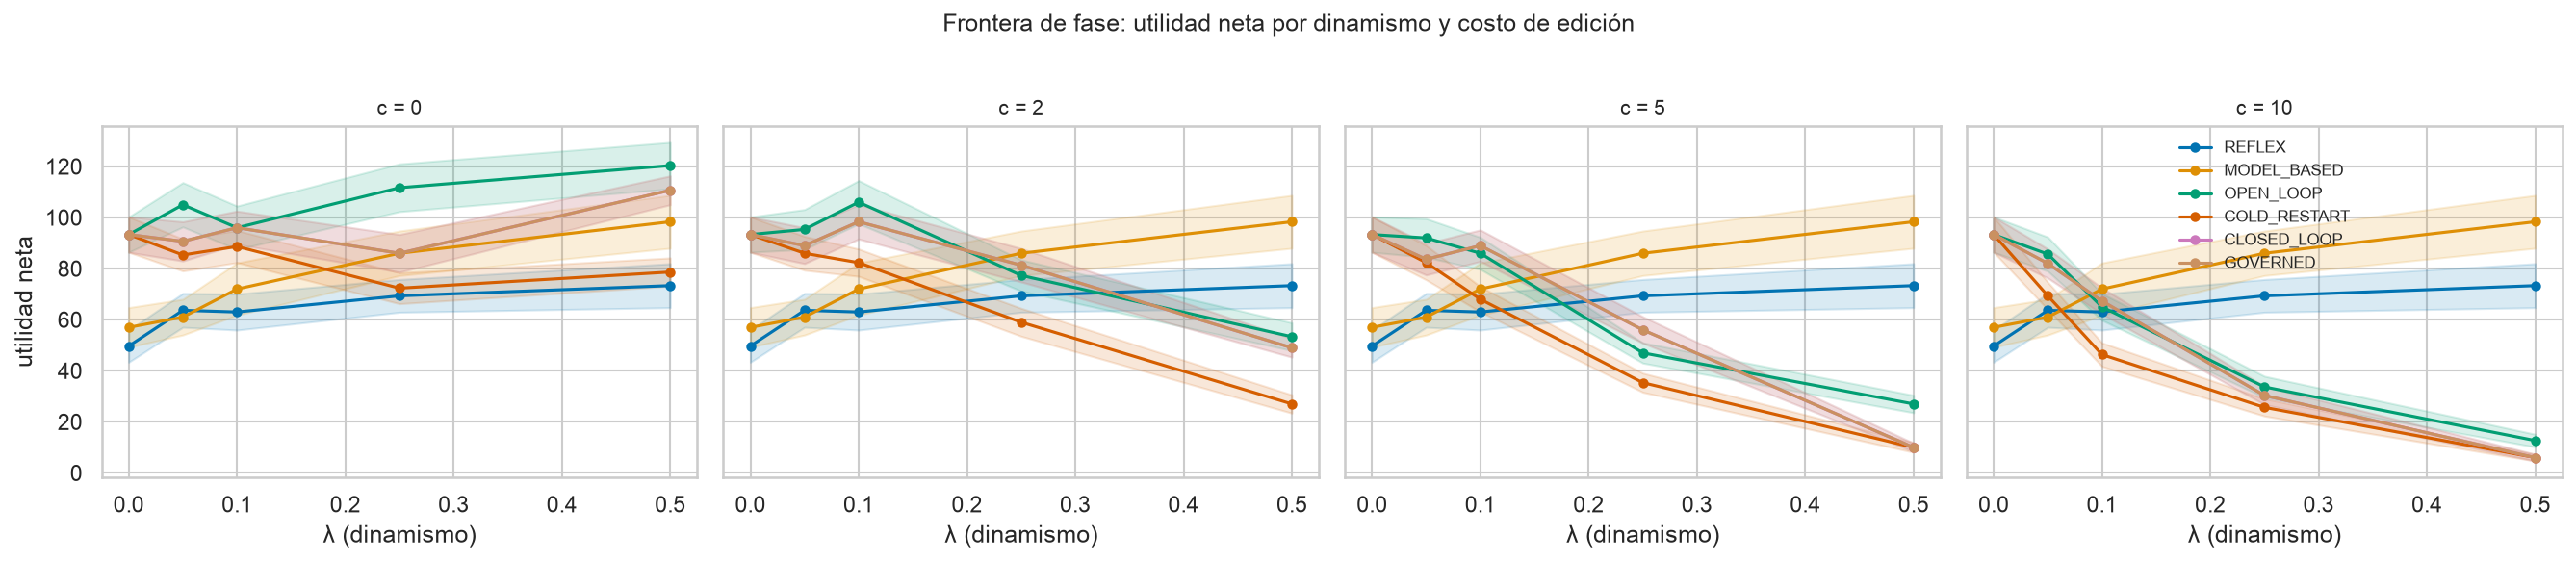
\includegraphics[width=\linewidth]{01-frontera}
  \caption{Frontera de fase: Utilidad neta contra $\lambda$ para las seis arquitecturas originales, un panel por $c$ ($p=0.9$, $r=3$, 3.600 corridas). La banda es el error estándar de la media. \CL{} y \GOV{} se superponen porque este barrido no fija presupuesto, y sin presupuesto \GOV{} es \CL. A medida que crecen $\lambda$ y $c$, las políticas que planifican se hunden mientras que \MB{} (reactiva con creencias, que nunca delibera) mejora con el dinamismo y no depende de $c$.}
  \label{fig:frontera}
\end{figure}

Primeramente, con $\lambda=0$ las cuatro políticas que planifican rinden exactamente lo mismo (93.3, que es el control 1) y casi duplican a las reactivas (49.7 el reflejo simple y 57.0 el basado en modelo), dado que sin dinamismo el plan nunca caduca y la previsión de A* para rodear obstáculos y encadenar objetivos vale más que cualquier reacción.

Progresivamente, a medida que crece $\lambda$, la comparación que motivaba el trabajo (reparar al ver la divergencia, \CL, contra esperar a que el plan falle, \OL) resulta mucho más pareja de lo esperado, pues la diferencia \OL$-$\CL{} va de $-9.0$ a $+25.7$ puntos según la celda y en 13 de las 16 celdas con $\lambda>0$ cae dentro de dos errores estándar. Las únicas celdas en que el lazo abierto se adelanta claramente son $\lambda=0.25$ con $c=0$ (111.7 contra 86.0) y $\lambda=0.5$ con $c=5$ (27.0 contra 10.0) y con $c=10$ (12.7 contra 6.0), y estas dos últimas están en un régimen donde todas las políticas que planifican ya colapsaron, mientras que en ninguna celda el lazo cerrado se adelanta más allá del ruido. Es decir que, con $r=3$ y cuando ambas cosas cuestan lo mismo, monitorear el plan no compra casi nada sobre replanificar solo al fallar.

Finalmente, lo que sí aparece con nitidez es otra frontera, la que separa deliberar de no deliberar en absoluto: El costo $c$ hunde a las políticas que planifican a medida que crece, y el hundimiento se acelera con $\lambda$, mientras que \MB{} no depende de $c$ y mejora con el dinamismo, de forma que pasa a ser la mejor política a $\lambda=0.5$ con cualquier $c\ge2$ (98.3 contra 53.3, 27.0 y 12.7 de la mejor que planifica con $c=2$, 5 y 10) y a $\lambda=0.25$ con $c\ge5$ (86.0 contra 56.0 y 33.7), con márgenes de entre tres y ocho errores estándar; con $c=2$ a $\lambda=0.25$ y con $c=10$ a $\lambda=0.1$ la diferencia cae dentro del ruido. Esa es la frontera que buscaba la pregunta, aunque no entre las dos políticas que se esperaba, pues el costo de reescritura a partir del cual la ventaja se invierte es el costo a partir del cual deja de convenir planificar, y no el que separa al lazo cerrado del abierto.

\begin{table}[htbp]
\centering
\footnotesize
\setlength{\tabcolsep}{4pt}
\begin{tabular}{@{}l rrrr c rrrr@{}}
\toprule
& \multicolumn{4}{c}{\OL{} $-$ \CL} & & \multicolumn{4}{c}{\MB{} $-$ mejor política con plan} \\
\cmidrule{2-5}\cmidrule{7-10}
$\lambda$ & $c=0$ & $c=2$ & $c=5$ & $c=10$ & & $c=0$ & $c=2$ & $c=5$ & $c=10$ \\
\midrule
0    & 0.0 & 0.0 & 0.0 & 0.0 & & \multicolumn{4}{c}{\textbf{−36.3 ± 9.6} (igual en todo $c$)} \\ \sepfilas
0.05 & +14.3 ± 8.2 & +6.3 ± 6.2 & +8.3 ± 6.7 & +3.7 ± 4.4 & & \textbf{−44.0 ± 8.1} & \textbf{−34.3 ± 7.2} & \textbf{−31.0 ± 7.0} & \textbf{−24.7 ± 6.8} \\ \sepfilas
0.1  & 0.0 ± 7.7 & +7.7 ± 8.2 & −3.0 ± 5.9 & −2.3 ± 4.8 & & \textbf{−24.0 ± 11.4} & \textbf{−34.0 ± 9.9} & −17.0 ± 8.8 & +4.7 ± 8.8 \\ \sepfilas
0.25 & \textbf{+25.7 ± 9.0} & −4.0 ± 6.7 & −9.0 ± 5.7 & +3.3 ± 5.7 & & \textbf{−25.7 ± 11.3} & +4.7 ± 9.4 & \textbf{+30.0 ± 10.1} & \textbf{+52.3 ± 9.2} \\ \sepfilas
0.5  & +9.7 ± 9.7 & +4.3 ± 5.3 & \textbf{+17.0 ± 3.8} & \textbf{+6.7 ± 3.1} & & −22.0 ± 11.2 & \textbf{+45.0 ± 11.7} & \textbf{+71.3 ± 9.6} & \textbf{+85.7 ± 10.5} \\
\bottomrule
\end{tabular}
\caption{Las dos diferencias que deciden la frontera (barrido \texttt{principal}). A la izquierda, lazo abierto menos lazo cerrado, casi siempre dentro del ruido. A la derecha, el agente que no delibera menos la política con plan de mayor media en cada celda, que pasa de perder por más de 20 puntos a ganar por más de 45 cuando $\lambda$ y $c$ crecen.}
\label{tab:frontera}
\end{table}

El mecanismo se lee en las métricas de las mismas corridas: A $\lambda=0.5$ con $c=5$, \CL{} pasa en promedio 282 de los 400 ticks deliberando y entrega 1.0 recurso, mientras que \OL, que replanifica menos veces, pasa 154 ticks deliberando y entrega 2.7, de forma que ambos gastan buena parte del horizonte pensando sobre un mundo que se mueve mientras piensan, y cada plan nace desactualizado, en tanto que el agente reactivo reevalúa en cada tick sin detenerse. De ahí se sigue además un matiz sobre la taxonomía de \textcite{russellNorvig2020}, pues su orden depende del entorno de tarea: \RX{} es el peor con $\lambda=0$, pero mejora con el dinamismo y a $\lambda=0.5$ con $c\ge2$ supera también a todo lo que planifica (73.3), de forma que planificar compra previsión y vende oportunismo, y cuál de las dos vale más es una propiedad del entorno y no del agente.

\textbf{Veredicto.} La hipótesis O1 se cumple solo en su parte trivial (con $\lambda=0$ las políticas que planifican empatan), pues con $r=3$ no aparece un umbral $\lambda^{*}$ a partir del cual reparar al ver la divergencia supere a esperar el fallo; la O2 se cumple en otro sentido del previsto, ya que $c$ resultó decisivo, pero para desplazar el punto desde el cual deja de convenir planificar.

\FloatBarrier
\subsection{Cuánto vale reparar en caliente frente a reiniciar en frío}\label{sec:res-caliente}

\CR{} modela a los sistemas que aplican las ediciones en la ejecución siguiente, en los que el trabajo en curso (la carga que el agente ya llevaba) se pierde, mientras que \CL{} repara el plan en caliente y conserva el progreso. Su diferencia es el argumento cuantitativo para decidir si un motor de ejecución agéntica debe reparar en caliente (figura~\ref{fig:caliente} y cuadro~\ref{tab:caliente}).

\begin{figure}[htbp]
  \centering
  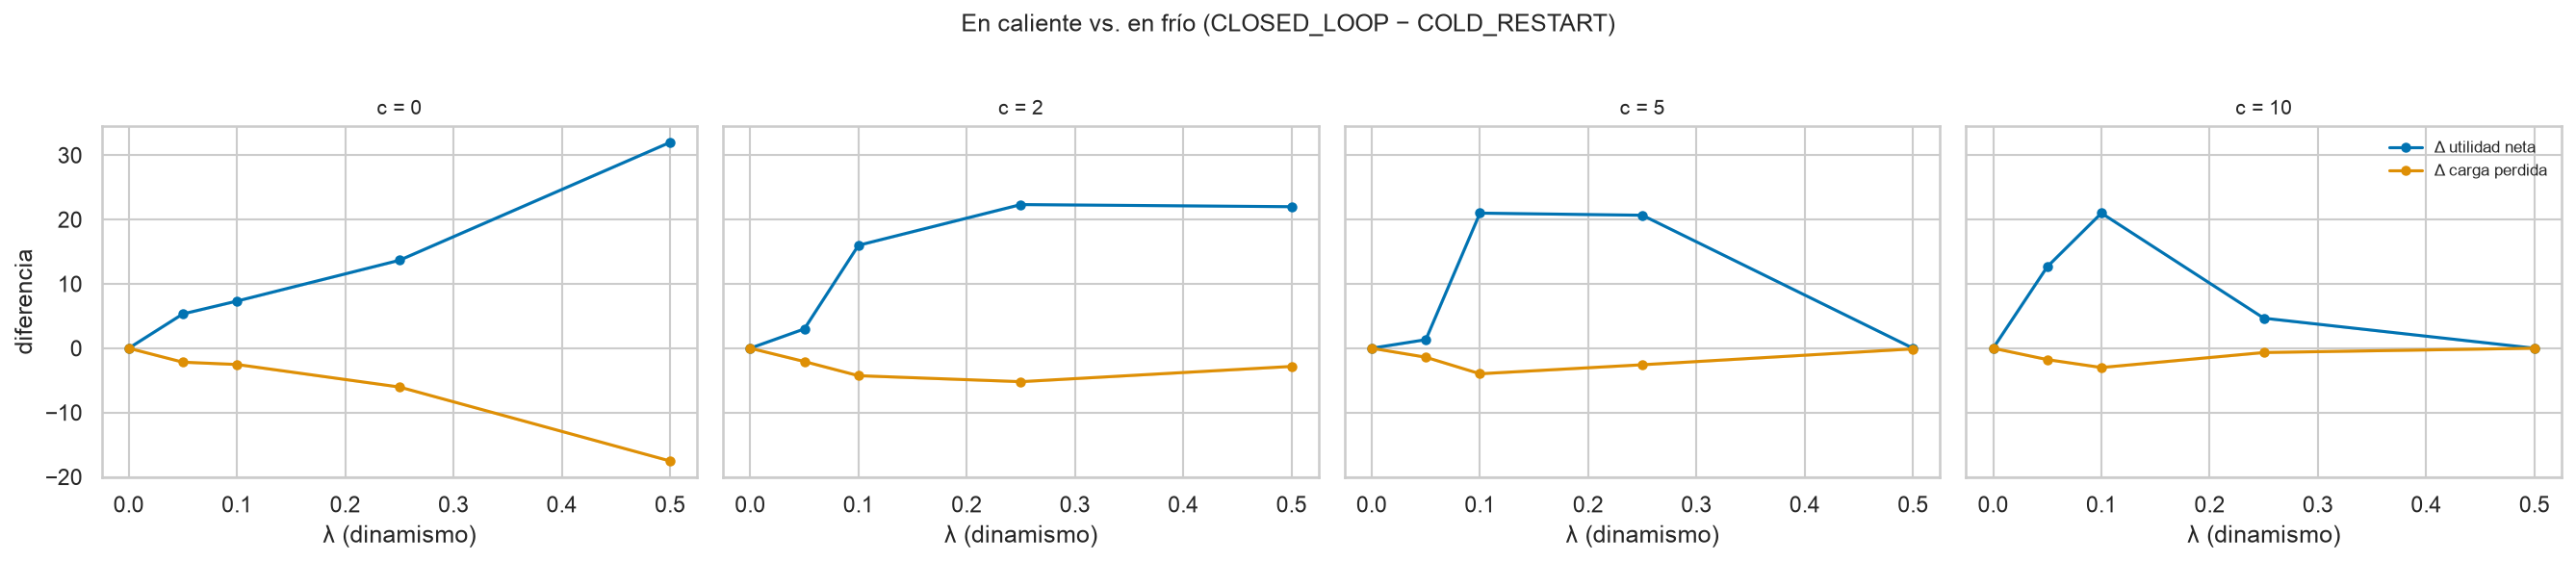
\includegraphics[width=\linewidth]{02-hot-vs-cold}
  \caption{Reparar en caliente menos reiniciar en frío (\CL$-$\CR), un panel por $c$: En azul la diferencia de utilidad neta y en naranja la de carga perdida por corrida. La ventaja es nula en un entorno estático, aparece con claridad desde $\lambda=0.1$ y se anula a $\lambda=0.5$ con $c\ge5$, donde las dos políticas colapsan.}
  \label{fig:caliente}
\end{figure}

\begin{table}[htbp]
\centering
\footnotesize
\begin{tabular}{@{}l rrrr@{}}
\toprule
$\lambda$ & $c=0$ & $c=2$ & $c=5$ & $c=10$ \\
\midrule
0.05 & +5.3 ± 5.0 & +3.0 ± 3.6 & +1.3 ± 5.1 & \textbf{+12.7 ± 4.3} \\ \sepfilas
0.1  & \textbf{+7.3 ± 3.1} & \textbf{+16.0 ± 5.6} & \textbf{+21.0 ± 5.3} & \textbf{+21.0 ± 5.7} \\ \sepfilas
0.25 & \textbf{+13.7 ± 4.2} & \textbf{+22.3 ± 4.1} & \textbf{+20.7 ± 5.6} & \textbf{+4.7 ± 2.1} \\ \sepfilas
0.5  & \textbf{+32.0 ± 5.7} & \textbf{+22.0 ± 4.1} & 0.0 ± 0.8 & 0.0 ± 0.0 \\
\bottomrule
\end{tabular}
\caption{Valor de reparar en caliente: \CL{} $-$ \CR{} en el barrido \texttt{principal} (con $\lambda=0$ la diferencia es exactamente cero).}
\label{tab:caliente}
\end{table}

La ventaja de reparar en caliente es cero en un entorno estático y aparece con claridad desde $\lambda=0.1$, donde vale entre $+7.3$ y $+21.0$ puntos según $c$ (de $+8$\,\% a $+45$\,\%); a $\lambda=0.25$ vale entre $+4.7$ y $+22.3$, y a $\lambda=0.5$ con deliberación gratuita llega a $+32.0$ puntos ($+41$\,\%), sostenida por una caída de 17.5 unidades por corrida en la carga perdida. Con visión total la ventaja es todavía mayor, pues en el barrido de observabilidad el reinicio en frío colapsa y \CL$-$\CR{} llega a \dif{+80.7}{7.0} a $\lambda=0.1$ (145.0 contra 64.3) y a \dif{+47.7}{4.3} a $\lambda=0.25$, que es la ventaja más grande de reparar en caliente en todo el trabajo. Cabe mencionar que esta es la conclusión que mejor sobrevivió a la corrección de la regla de costo, e incluso se fortaleció (a $\lambda=0.1$ con $c=5$ pasó de $+4$ a $+21$ puntos), lo cual tiene sentido, porque ahora las dos políticas pagan lo mismo por cada replanificación y lo único que las separa es el trabajo en curso que una conserva y la otra tira.

Vale la pena matizar dos cosas. Primeramente, la relación con $c$ no es monótona, pues a $\lambda=0.25$ el máximo está en $c=2$ y no en $c=0$, y a $\lambda=0.1$ la ventaja crece con $c$ en vez de caer, de forma que lo defendible es el signo de la ventaja y su aparición desde $\lambda=0.1$, y no el valor de cada celda (el porcentaje, además, se infla cuando el reinicio en frío rinde poco, como el $+81$\,\% de $\lambda=0.5$ con $c=2$, que son 22 puntos sobre una base de 27). Finalmente, la ventaja se anula a $\lambda=0.5$ con $c\ge5$, no porque reiniciar en frío sea bueno ahí, sino porque ambas políticas colapsan (10.0 contra 10.0 con $c=5$), de forma que no queda trabajo en curso que perder.

\textbf{Veredicto.} La hipótesis O5 se confirma: Construir la reparación en caliente compensa en cuanto el entorno cambia con alguna frecuencia (desde $\lambda=0.1$ en este modelo), siempre que deliberar no sea tan caro que el agente deje de completar entregas.

\FloatBarrier
\subsection{La competencia del replanificador}\label{sec:res-competencia}

La competencia $p$ es la probabilidad de que la reparación del oráculo sea la óptima, y su fallo no es ruido sino un plan plausible y equivocado (figura~\ref{fig:competencia}). La competencia sí mueve el resultado, aunque no del modo esperado, pues la política más sensible a $p$ resultó ser el lazo abierto y no el cerrado: Entre $p=0.5$ y $p=1$, \OL{} pasa de 36.7 a 61.0 a $\lambda=0.25$ y de 16.3 a 34.7 a $\lambda=0.5$, mientras que \CL{} pasa de 48.3 a 59.7 a $\lambda=0.25$ y se queda plano a $\lambda=0.5$ (entre 10.0 y 14.0), donde lo que lo hunde es la cantidad de reparaciones que paga y no su calidad; a $\lambda=0.1$ todas las pendientes caen dentro del ruido.

\begin{figure}[htbp]
  \centering
  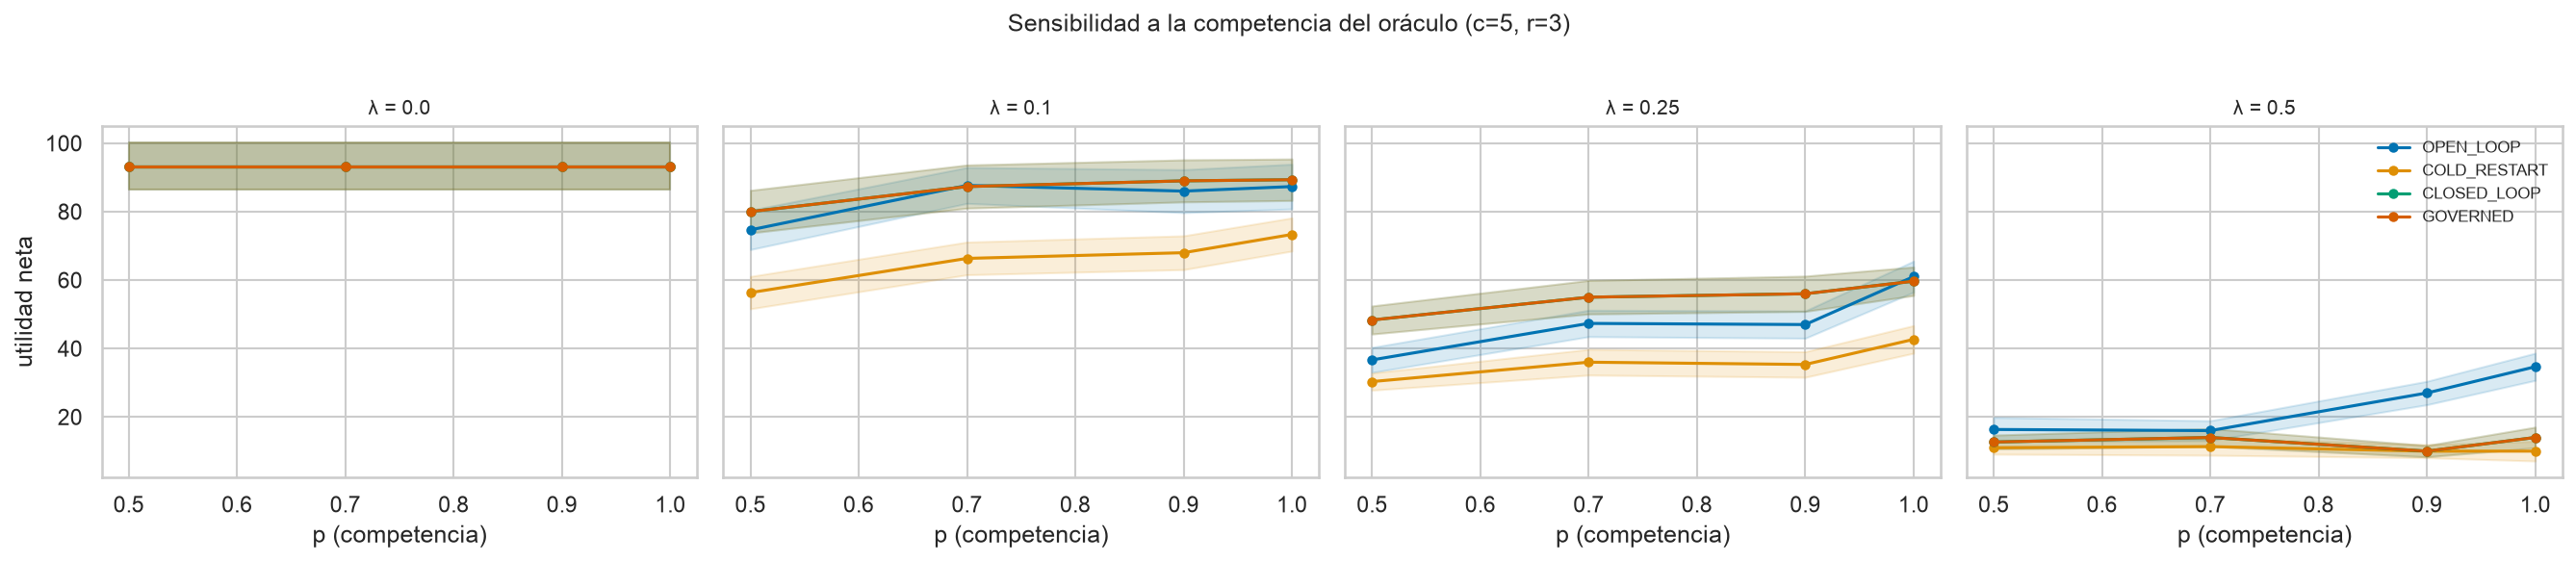
\includegraphics[width=\linewidth]{03-competencia}
  \caption{Sensibilidad a la competencia del oráculo ($c=5$, $r=3$), un panel por $\lambda$. El lazo abierto (azul) es el que más depende de $p$; el cerrado y el gobernado (superpuestos) apenas se mueven, y a $\lambda=0.5$ el abierto se adelanta solo desde $p=0.9$.}
  \label{fig:competencia}
\end{figure}

El orden entre ambas cambia entonces con $p$: Con un replanificador mediocre ($p=0.5$) el lazo cerrado rinde más a $\lambda=0.25$ (\dif{+11.7}{4.7} sobre el abierto), con uno perfecto empatan (59.7 contra 61.0), y a $\lambda=0.5$ el lazo abierto se adelanta solo desde $p=0.9$ (\dif{+17.0}{3.8}, y \dif{+20.7}{4.4} con $p=1$). Una lectura plausible, que no se verificó con una métrica específica, es que un error del replanificador le cuesta al lazo abierto un viaje completo hasta la celda equivocada antes de descubrirlo, mientras que el lazo cerrado lo corrige en la siguiente observación, aunque pagando otra reparación, de forma que la calidad de cada reparación pesa más para quien repara poco. Hay además un límite estructural, pues cuando el agente pide una reparación sin ver su objetivo el oráculo no puede acertar, de modo que con $r=3$ una parte de las consultas no depende de $p$.

\textbf{Veredicto.} La hipótesis O3 no se sostiene: El control 3 pasa solo por el signo y, en el barrido de competencia, un replanificador mediocre favorece incluso al lazo cerrado frente al abierto, de forma que en este barrido no existe una competencia mínima a partir de la cual reparar al ver la divergencia supere a esperar el fallo.

\FloatBarrier
\subsection{Observabilidad parcial}\label{sec:res-observabilidad}

El radio $r$ modela qué parte del entorno tiene el agente en su contexto, y la métrica que importa no es si el agente se entera de una divergencia sino cuándo (figura~\ref{fig:observabilidad} y cuadro~\ref{tab:observabilidad}). La ceguera es casi nula en todos los radios (a lo sumo 3\,\% en promedio por radio y 4.4\,\% en el peor caso, \OL{} con $r=1$), justo como predecía el diseño, pues las divergencias no se pierden sino que se detectan tarde: La latencia promedio baja de 1.24–1.27 ticks con $r=1$ y $r=3$ (entre los cuales no hay un orden claro) a 0.72 con $r=\infty$.

\begin{figure}[htbp]
  \centering
  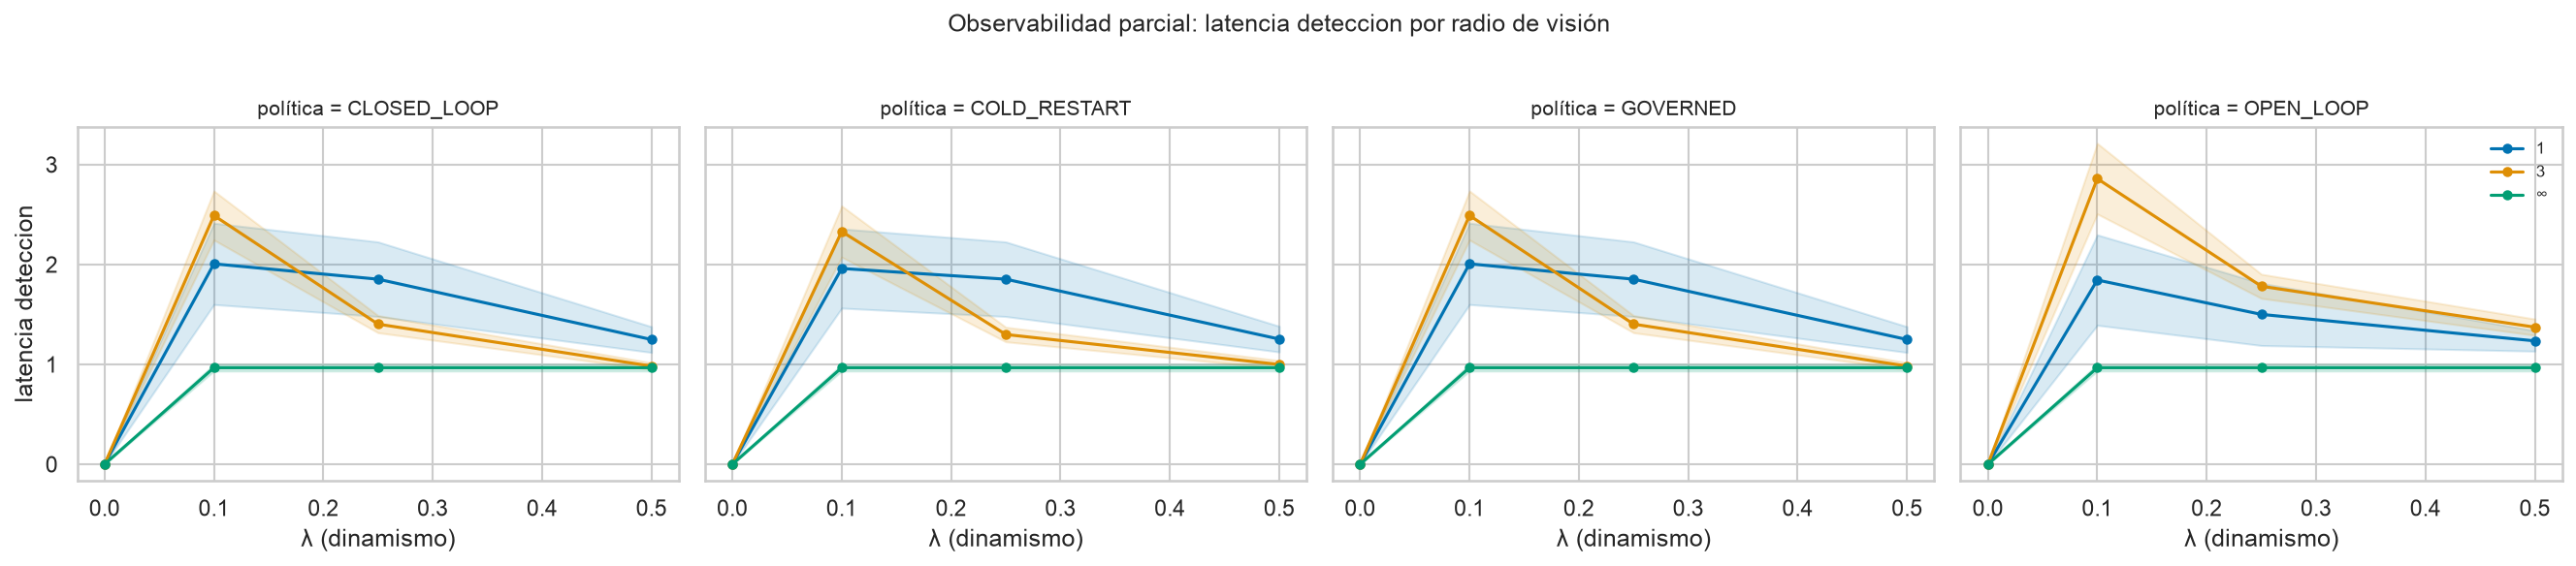
\includegraphics[width=\linewidth]{04-observabilidad}
  \caption{Latencia de detección (ticks entre que ocurre una divergencia y el agente la nota) contra $\lambda$, una línea por radio y un panel por política ($c=5$, $p=0.9$). Con visión total la latencia es la mínima posible; con $r=1$ y $r=3$ el agente camina en promedio uno o dos ticks más hacia una celda donde el recurso ya no está.}
  \label{fig:observabilidad}
\end{figure}

\begin{table}[htbp]
\centering
\footnotesize
\begin{tabular}{@{}l rrrr rrr@{}}
\toprule
$r$ & Latencia & Ceguera & Ediciones & Utilidad & $U(\lambda=0)$ & \OL{} & \CL{} \\
\midrule
1        & 1.24 & 0.03 & 1.46  & 48.1  & 47.0  & 48.0  & 47.9 \\ \sepfilas
3        & 1.27 & 0.02 & 10.95 & 59.8  & 93.3  & 63.3  & 62.1 \\ \sepfilas
$\infty$ & 0.72 & 0.00 & 14.81 & 110.2 & 261.0 & 129.5 & 114.5 \\
\bottomrule
\end{tabular}
\caption{Observabilidad parcial, promedios por radio sobre $\lambda \in \{0, 0.1, 0.25, 0.5\}$ y las cuatro políticas con plan ($c=5$). Las dos últimas columnas son la utilidad media del lazo abierto y del cerrado.}
\label{tab:observabilidad}
\end{table}

La utilidad media sube de 48.1 con $r=1$ a 59.8 con $r=3$ y 110.2 con $r=\infty$, pero la tesis de una versión anterior del modelo (que la observabilidad dominaba todo lo demás y que con visión total la replanificación ganaba) no sobrevivió a la corrección, y la lectura actual tiene tres partes:

\begin{itemize}[leftmargin=1.4em, itemsep=0.2em]
  \item \textbf{La observabilidad fija el nivel de todas las políticas por igual:} Con $\lambda=0$, donde nadie replanifica, las cuatro rinden 47.0 con $r=1$, 93.3 con $r=3$ y 261.0 con $r=\infty$, de forma que buena parte del salto entre radios es que ver más permite encontrar más recursos, lo cual no dice nada sobre si conviene reescribir el plan.
  \item \textbf{Con $r=1$ las políticas son indistinguibles:} En todo $\lambda$ quedan a menos de 4 puntos entre sí, con un error estándar de ese mismo orden, dado que con tan poca visión el agente apenas edita su plan (entre 1.0 y 2.6 ediciones por corrida).
  \item \textbf{Con visión total las diferencias se amplían, pero no a favor de reparar al ver la divergencia:} El lazo abierto supera al cerrado a $\lambda=0.25$ (72.0 contra 52.0, \dif{+20.0}{5.1}) y a $\lambda=0.5$ (34.0 contra 0.0, \dif{+34.0}{4.5}), porque viéndolo todo el lazo cerrado detecta cada divergencia en cuanto ocurre y paga $c$ por cada una, de forma que a $\lambda=0.5$ pasa 372 de los 400 ticks deliberando y no completa ninguna entrega, mientras que el abierto delibera 171 ticks y entrega 3.4 recursos.
\end{itemize}

Es decir que la observabilidad amplifica lo que el costo de deliberar decide: Con deliberación gratuita y oráculo perfecto (el control 2, que también es con $r=\infty$) el lazo cerrado sí domina, por $+45$ y $+56$ puntos a $\lambda=0.25$ y $0.5$, mientras que con $c=5$ y $p=0.9$ pierde en esos mismos $\lambda$. Vale la pena anotar con honestidad que entre esos dos puntos cambian a la vez $c$ y $p$, por lo que la inversión no se puede atribuir solo al costo (aunque §\ref{sec:res-competencia} sugiere que $p$ pesa poco sobre el lazo cerrado), y que el barrido de observabilidad solo tiene $c=5$.

\FloatBarrier
\subsection{Gobernanza: acotar las reparaciones}\label{sec:res-gobernanza}

\GOV{} es reparación en caliente con un presupuesto de $B$ reparaciones proactivas, de forma que agotado el presupuesto se comporta exactamente como el lazo abierto, y el barrido va desde $B=0$ (el lazo abierto, control 6) hasta $B=25$, que en la práctica coincide con \CL{} (figura~\ref{fig:gobernanza} y cuadro~\ref{tab:gobernanza}).

\begin{figure}[htbp]
  \centering
  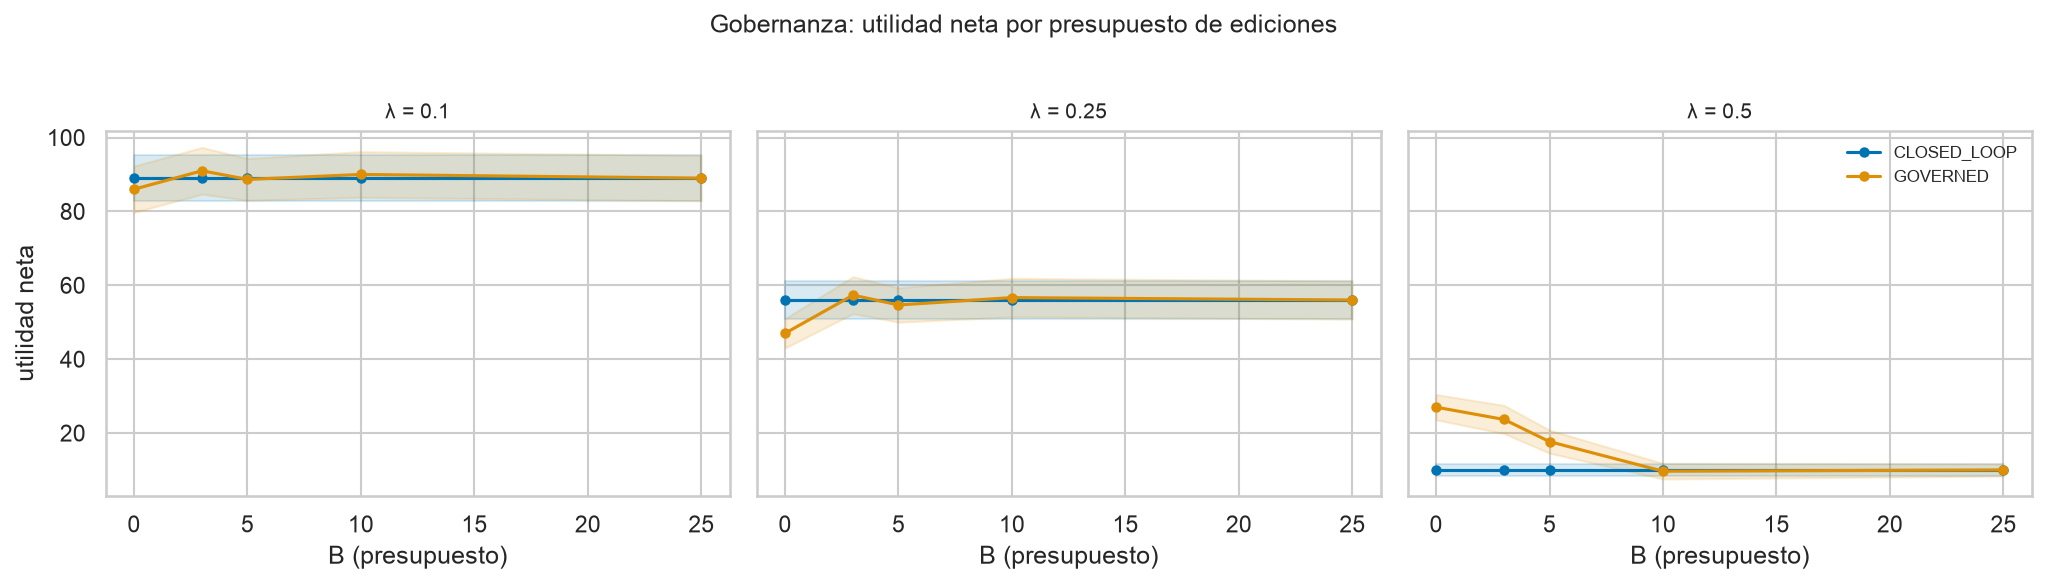
\includegraphics[width=\linewidth]{05-gobernanza}
  \caption{Utilidad neta contra el presupuesto $B$ de reparaciones proactivas, un panel por $\lambda$ ($c=5$, $r=3$). \CL{} no tiene presupuesto y aparece como referencia horizontal; $B=0$ es exactamente \OL. Solo a $\lambda=0.5$ el presupuesto separa a \GOV{} del lazo cerrado, y ahí el mejor presupuesto es cero.}
  \label{fig:gobernanza}
\end{figure}

\begin{table}[htbp]
\centering
\footnotesize
\begin{tabular}{@{}l rrr rrr@{}}
\toprule
& \multicolumn{3}{c}{Utilidad neta} & \multicolumn{3}{c}{Mecanismo a $\lambda=0.5$} \\
\cmidrule(lr){2-4}\cmidrule(l){5-7}
& $\lambda=0.1$ & $\lambda=0.25$ & $\lambda=0.5$ & Desperdiciadas & Ticks deliberando & Por fallo \\
\midrule
\GOV, $B=0$ ($\equiv$ \OL) & 86.0 & 47.0 & 27.0 & 10.1  & 153.6 & 30.6 \\ \sepfilas
\GOV, $B=3$  & 91.0 & 57.3 & 23.7 & 50.7  & 187.7 & 22.4 \\ \sepfilas
\GOV, $B=5$  & 88.7 & 54.7 & 17.7 & 75.3  & 206.7 & 18.9 \\ \sepfilas
\GOV, $B=10$ & 90.0 & 56.7 & 9.7  & 129.0 & 248.6 & 10.4 \\ \sepfilas
\GOV, $B=25$ & 89.0 & 56.0 & 10.0 & 181.1 & 282.0 & 1.2 \\ \sepfilas
\CL          & 89.0 & 56.0 & 10.0 & 181.8 & 282.2 & 1.1 \\
\bottomrule
\end{tabular}
\caption{Gobernanza por presupuesto (medias por corrida, $c=5$, $r=3$). Las tres últimas columnas son, a $\lambda=0.5$, las ediciones desperdiciadas, los ticks deliberando y las replanificaciones forzadas por un fallo.}
\label{tab:gobernanza}
\end{table}

El presupuesto no rescata al lazo cerrado del modo en que parecía en la versión anterior del modelo, cuyo «rescate» era en su mayor parte el mismo artefacto de la replanificación gratuita. A $\lambda=0.1$ el presupuesto no mueve nada medible (todas las variantes quedan entre 86.0 y 91.0, con un error estándar de unos 6 puntos); a $\lambda=0.25$ un presupuesto pequeño recupera el nivel del lazo cerrado (57.3 con $B=3$ contra 56.0), y lo que rinde menos es no reparar nunca de forma proactiva (47.0 con $B=0$), aunque esa diferencia de unos 10 puntos apenas supera dos errores estándar; y a $\lambda=0.5$ acotar sí ayuda frente al lazo cerrado sin acotar (23.7 con $B=3$ contra 10.0), pero la utilidad decrece con $B$ y el mejor presupuesto es cero (27.0, aunque su diferencia con $B=3$ cae dentro del ruido), de forma que lo que mejora el rendimiento no es una cuota óptima sino reparar menos, y todo el régimen queda muy por debajo del 98.3 de \MB.

El mecanismo confirma que el \emph{thrashing} es real y que el presupuesto lo corta, pues a $\lambda=0.5$ las ediciones desperdiciadas caen de 181.8 por corrida en el lazo cerrado a 50.7 con $B=3$ y a 10.1 con $B=0$, y los ticks deliberando de 282 a 188 y 154. Cabe mencionar que acotar las reparaciones proactivas no elimina las replanificaciones sino que las desplaza hacia las forzadas por un fallo (de 1.1 por corrida a 22.4 con $B=3$ y 30.6 con $B=0$), que también se pagan.

\textbf{Veredicto.} La hipótesis O4 se cumple solo en parte: Acotar evita el peor caso cuando el entorno cambia rápido y deliberar es caro, pero no hay una cuota óptima que rescate al agente, y el presupuesto explica a lo sumo el 0.3\,\% de la varianza de la utilidad (§\ref{sec:res-sensibilidad}).

\FloatBarrier
\subsection{Robustez al orden de activación}\label{sec:res-orden}

Por defecto el recolector actúa en cada tick antes de que los recursos deriven, lo cual fija a mano la sincronización de las divergencias, y como la sesión de predador–presa del curso advierte, quien mueve primero gana o pierde información de forma sistemática, de modo que es una amenaza de validez interna. El barrido \texttt{orden} repite un subconjunto de \texttt{principal} sorteando el orden en cada tick, y lo que se compara es el signo de las tres diferencias que sostienen las conclusiones (cuadro~\ref{tab:orden}).

\begin{table}[htbp]
\centering
\footnotesize
\setlength{\tabcolsep}{4pt}
\begin{tabular}{@{}ll rr rr rr@{}}
\toprule
& & \multicolumn{2}{c}{Caliente $-$ frío} & \multicolumn{2}{c}{Abierto $-$ cerrado} & \multicolumn{2}{c}{\ab{MB} $-$ mejor con plan} \\
\cmidrule(lr){3-4}\cmidrule(lr){5-6}\cmidrule(l){7-8}
$\lambda$ & $c$ & Fijo & Sorteado & Fijo & Sorteado & Fijo & Sorteado \\
\midrule
0.1  & 2 & \textbf{+16.0 ± 5.6} & \textbf{+9.3 ± 3.3} & +7.7 ± 8.2 & +8.7 ± 4.6 & −34.0 & −27.7 \\ \sepfilas
0.1  & 5 & \textbf{+21.0 ± 5.3} & \textbf{+9.7 ± 3.9} & −3.0 ± 5.9 & \textbf{+13.3 ± 5.1} & −17.0 & −22.7 \\ \sepfilas
0.25 & 2 & \textbf{+22.3 ± 4.1} & \textbf{+15.3 ± 5.0} & −4.0 ± 6.7 & \textbf{+12.3 ± 5.1} & +4.7 & −12.0 \\ \sepfilas
0.25 & 5 & \textbf{+20.7 ± 5.6} & \textbf{+16.0 ± 3.6} & −9.0 ± 5.7 & +5.3 ± 6.2 & +30.0 & +16.3 \\ \sepfilas
0.5  & 2 & \textbf{+22.0 ± 4.1} & \textbf{+26.7 ± 4.4} & +4.3 ± 5.3 & +3.7 ± 5.0 & +45.0 & +33.7 \\ \sepfilas
0.5  & 5 & 0.0 ± 0.8 & \textbf{+3.3 ± 1.2} & \textbf{+17.0 ± 3.8} & \textbf{+14.0 ± 5.2} & +71.3 & +57.7 \\
\bottomrule
\end{tabular}
\caption{Las tres diferencias que sostienen las conclusiones, con el orden de activación fijo (\texttt{principal}) y sorteado (\texttt{orden}), con $r=3$ y $p=0.9$. La última columna compara medias, sin error estándar.}
\label{tab:orden}
\end{table}

Las dos conclusiones cualitativas que sostienen el trabajo no dependen de quién mueve primero. Primeramente, en la comparación entre caliente y frío el signo coincide en 5 de las 6 celdas, y la sexta no es una excepción real, pues con orden fijo a $\lambda=0.5$ y $c=5$ las dos políticas colapsan y empatan, mientras que con orden sorteado la ventaja del caliente es pequeña pero positiva; con orden sorteado la ventaja es positiva en las seis celdas, aunque más chica que con orden fijo a $\lambda=0.1$ (+9.3 y +9.7 contra +16.0 y +21.0), lo cual deja la conclusión intacta en signo y la vuelve prudente en magnitud. Progresivamente, en la comparación entre no planificar y planificar el signo coincide también en 5 de 6 celdas, y la que cambia ($\lambda=0.25$ con $c=2$) es justamente la que el barrido principal ya había dejado dentro del ruido, mientras que donde \MB{} ganaba sigue ganando, por entre $+16.3$ y $+57.7$ puntos. Finalmente, la diferencia entre lazo abierto y cerrado cambia de signo en 3 de 6 celdas, que es lo que cabe esperar de una diferencia que ya estaba dentro de dos errores estándar en casi todo el rango; vale la pena anotar que con orden sorteado el lazo abierto queda arriba en las seis celdas, y en tres de ellas por más de dos errores estándar, de modo que si el orden mueve algo es a favor de no monitorear.

\textbf{Veredicto.} La hipótesis se confirma para las dos conclusiones cualitativas (reparar en caliente supera al frío con $\lambda>0$, y no planificar gana con $\lambda$ alto y deliberación cara), mientras que la comparación entre lazo abierto y lazo cerrado, que ya era la más frágil, no tiene un signo estable.

\FloatBarrier
\subsection{Dinámica: cuándo se separan las políticas}\label{sec:res-dinamica}

Los barridos guardan solo el valor final de cada corrida, de modo que no dicen \emph{cuándo} se separan las políticas. Las series temporales repiten la rebanada central de la frontera ($c=5$, $r=3$, $p=0.9$) con cinco políticas, cuatro valores de $\lambda$ y 30 semillas, guardando una fila cada cinco ticks. El plan de esta extensión suponía que las políticas se separan en un momento identificable, por ejemplo cuando se acumulan las primeras divergencias, y lo que se encontró es otra cosa (cuadros~\ref{tab:dinamica} y~\ref{tab:separacion}).

\begin{table}[htbp]
\centering
\footnotesize
\begin{tabular}{@{}l ccccc@{}}
\toprule
$\lambda$ & \RX & \MB & \OL & \CR & \CL \\
\midrule
0    & 1.8 / 3.2 / 5.0 & 1.7 / 3.7 / 5.7 & 2.7 / 5.0 / 9.3 & 2.7 / 5.0 / 9.3 & 2.7 / 5.0 / 9.3 \\ \sepfilas
0.1  & 2.5 / 3.9 / 6.3 & 2.6 / 4.4 / 7.2 & 2.3 / 4.5 / 8.6 & 2.2 / 4.0 / 6.8 & 2.4 / 4.6 / 8.9 \\ \sepfilas
0.25 & 2.9 / 4.4 / 6.9 & 3.3 / 5.3 / 8.6 & 1.4 / 2.4 / 4.7 & 1.3 / 1.9 / 3.5 & 1.6 / 3.0 / 5.6 \\ \sepfilas
0.5  & 2.7 / 4.9 / 7.3 & 3.2 / 5.8 / 9.8 & 0.6 / 1.3 / 2.7 & 0.3 / 0.6 / 1.0 & 0.3 / 0.6 / 1.0 \\
\bottomrule
\end{tabular}
\caption{Entregas acumuladas medias en los ticks 100, 200 y 400 ($c=5$, $r=3$, 600 corridas). El crecimiento es casi lineal en todas las celdas.}
\label{tab:dinamica}
\end{table}

\begin{table}[htbp]
\centering
\footnotesize
\begin{tabular}{@{}l llll@{}}
\toprule
$\lambda$ & \ab{MB}$-$\ab{CL} & \ab{MB}$-$\ab{OL} & \ab{CL}$-$\ab{CR} & \ab{OL}$-$\ab{CL} \\
\midrule
0    & tick 50 (−3.6 ± 1.0) & tick 50 (−3.6 ± 1.0) & nunca (0.0) & nunca (0.0) \\ \sepfilas
0.1  & nunca (−1.7 ± 0.9) & nunca (−1.4 ± 1.1) & tick 130 (+2.1 ± 0.5) & nunca (−0.3 ± 0.6) \\ \sepfilas
0.25 & tick 30 (+3.0 ± 1.0) & tick 25 (+3.9 ± 0.9) & tick 105 (+2.1 ± 0.6) & nunca (−0.9 ± 0.6) \\ \sepfilas
0.5  & tick 15 (+8.8 ± 1.0) & tick 15 (+7.1 ± 1.0) & nunca (+0.0 ± 0.1) & tick 170 (+1.7 ± 0.4) \\
\bottomrule
\end{tabular}
\caption{Primer tick desde el cual la diferencia pareada de entregas supera dos errores estándar y ya no vuelve a bajar hasta el final; entre paréntesis, la diferencia en entregas en el tick 400.}
\label{tab:separacion}
\end{table}

La separación no es un evento sino un ritmo. Las curvas de entregas acumuladas son casi rectas desde el tick 50, de forma que cada política entrega a un paso que fija $\lambda$ y lo mantiene (\CL{} a $\lambda=0.1$ entrega 2.1 recursos por cada 100 ticks tanto entre los ticks 50 y 200 como entre los 200 y 400, y \OL{} a $\lambda=0.5$, 0.7 en ambos tramos), por lo que las diferencias finales de la frontera son pendientes distintas acumuladas durante 400 ticks y no el resultado de un episodio puntual. Con $\lambda$ alto, no planificar se adelanta casi de inmediato (\MB{} supera al lazo cerrado desde el tick 15 con $\lambda=0.5$ y desde el 30 con $\lambda=0.25$), lo cual es la frontera de §\ref{sec:res-frontera} vista en el tiempo; reparar en caliente, en cambio, tarda en pagar, pues su ventaja sobre el frío se separa del ruido recién desde el tick 130 con $\lambda=0.1$ y el 105 con $\lambda=0.25$, cuando el agente ya acumuló trabajo en curso que un reinicio tiraría. Los ticks deliberando también crecen en línea recta (a $\lambda=0.5$, \CL{} delibera 64 de los primeros 100 ticks y 282 de los 400), de modo que el \emph{thrashing} no es una crisis que llegue en algún momento sino un impuesto que se cobra desde el principio y a ritmo constante.

\FloatBarrier
\subsection{El agente basado en conocimiento}\label{sec:res-kb}

La figura~\ref{fig:conocimiento} reúne las cinco políticas del barrido \texttt{conocimiento}, una faceta por radio, y el cuadro~\ref{tab:kb} pone en números los contrastes de H1, de la ablación, de H1b y de H3. Primero los controles exactos (cuadro~\ref{tab:controles}), que pasan sin una sola corrida distinta: Con visión total y el horizonte \ahora{} la región lógica es exactamente el monitor de \CL{} (H2), y añadir las dos políticas nuevas no tocó a las demás.

\begin{figure}[htbp]
  \centering
  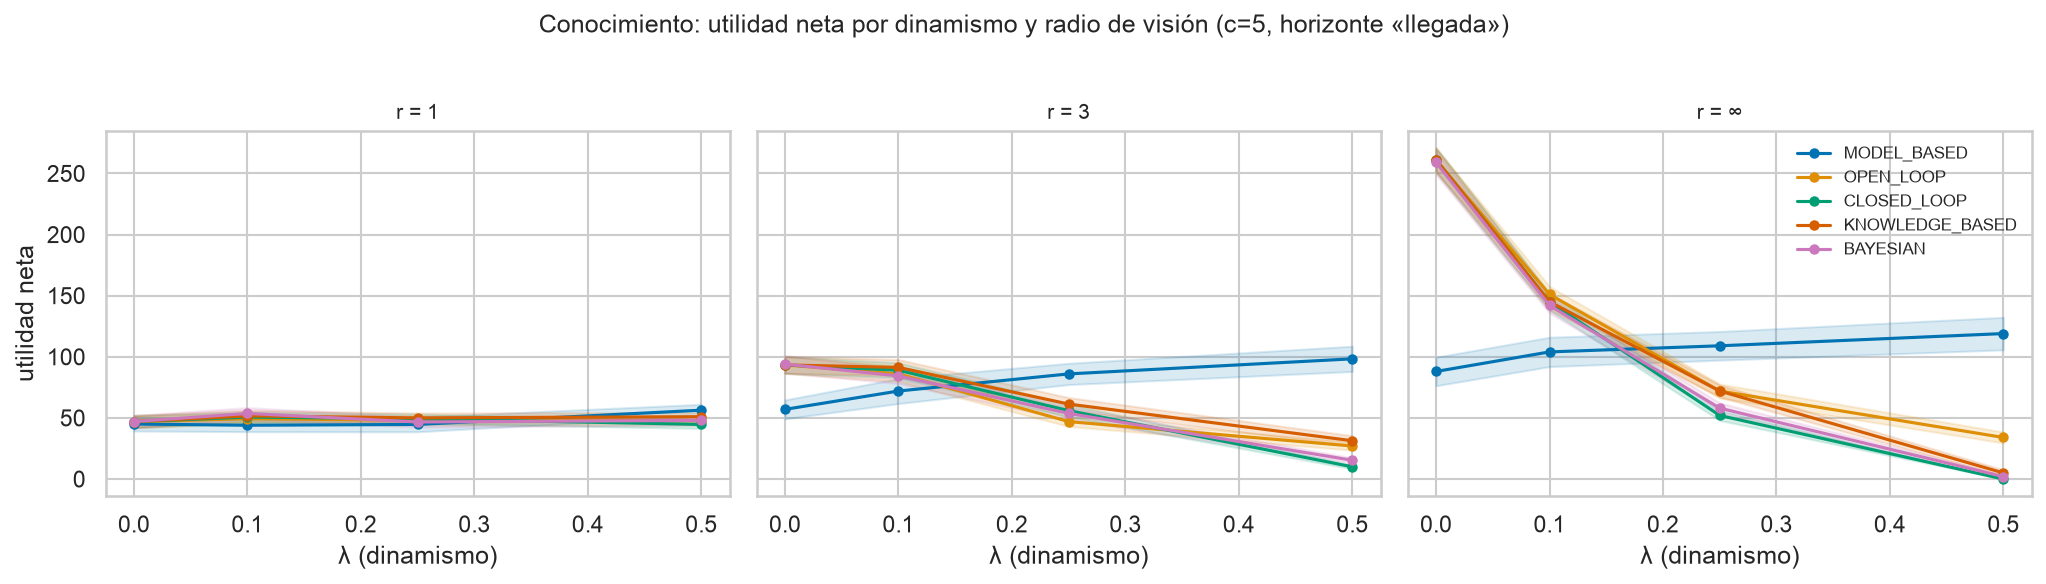
\includegraphics[width=\linewidth]{06-conocimiento}
  \caption{Utilidad neta de las cinco políticas del barrido \texttt{conocimiento} ($c=5$, horizonte \llegada), una faceta por radio. Con $r=1$ todas quedan juntas; con $r=3$ \KB{} queda por encima del lazo cerrado a $\lambda=0.5$ pero muy por debajo de \MB; con visión total ninguna política con plan resiste el dinamismo alto.}
  \label{fig:conocimiento}
\end{figure}

\begin{table}[htbp]
\centering
\footnotesize
\setlength{\tabcolsep}{3.5pt}
\begin{tabular}{@{}l rrrr rrr@{}}
\toprule
& \multicolumn{4}{c}{Contrastes ($r=3$, consulta gratuita)} & \multicolumn{3}{c}{H3: \ab{KB}$-$\ab{CL} con costo por consulta} \\
\cmidrule(lr){2-5}\cmidrule(l){6-8}
$\lambda$ & H1: \ab{KB}$-$\ab{CL} & \ab{KB} \ahora{}$-$\ab{CL} & \ab{KB}$-$\ab{OL} & \ab{KB}$-$\ab{MB} & 1 tick & 2 ticks & 5 ticks \\
\midrule
0.1  & +2.3 ± 6.1 & +5.7 ± 4.1 & +5.3 ± 4.7 & +19.3 ± 10.6 & −5.3 ± 5.5 & −9.0 ± 4.8 & \textbf{−32.3 ± 5.6} \\ \sepfilas
0.25 & +5.3 ± 6.2 & −3.0 ± 5.1 & \textbf{+14.3 ± 4.2} & \textbf{−24.7 ± 9.8} & \textbf{−17.3 ± 5.6} & \textbf{−30.3 ± 5.8} & \textbf{−36.7 ± 5.6} \\ \sepfilas
0.5  & \textbf{+21.3 ± 3.8} & −1.3 ± 2.6 & +4.3 ± 5.3 & \textbf{−67.0 ± 10.5} & −2.3 ± 2.0 & −3.7 ± 1.9 & \textbf{−4.7 ± 2.0} \\
\bottomrule
\end{tabular}
\caption{Agente basado en conocimiento con $r=3$ y $c=5$. La segunda columna es la ablación con horizonte \ahora, que conserva la elección de objetivo por peor caso y vuelve la decisión de reparar idéntica al monitor del lazo cerrado.}
\label{tab:kb}
\end{table}

\begin{table}[htbp]
\centering
\footnotesize
\begin{tabular}{@{}ll rrrrrr@{}}
\toprule
$\lambda$ & Política & Por fallo & Proactivas & Desperdiciadas & Ticks deliberando & Consultas & Entregas \\
\midrule
0.1  & \OL & 10.6 & 0.0 & 3.6 & 53.5 & 0.0 & 8.6 \\
     & \CL & 1.6 & 7.7 & 7.1 & 56.2 & 0.0 & 8.9 \\
     & \KB & 7.3 & 2.8 & 4.4 & 53.7 & 16.0 & 9.1 \\
     & \BY & 3.3 & 6.2 & 5.9 & 56.2 & 23.1 & 8.4 \\ \sepfilas
0.25 & \OL & 21.6 & 0.0 & 7.7 & 108.8 & 0.0 & 4.7 \\
     & \CL & 1.6 & 9.7 & 35.5 & 109.9 & 0.0 & 5.6 \\
     & \KB & 9.3 & 6.5 & 24.1 & 115.5 & 58.9 & 6.1 \\
     & \BY & 7.1 & 11.9 & 38.9 & 145.6 & 75.7 & 5.4 \\ \sepfilas
0.5  & \OL & 30.6 & 0.0 & 10.1 & 153.6 & 0.0 & 2.7 \\
     & \CL & 1.1 & 13.7 & 181.8 & 282.2 & 0.0 & 1.0 \\
     & \KB & 6.6 & 9.5 & 97.4 & 219.2 & 192.1 & 3.1 \\
     & \BY & 5.7 & 16.3 & 145.8 & 265.1 & 208.1 & 1.5 \\
\bottomrule
\end{tabular}
\caption{Mecanismo con $r=3$ y $c=5$ (medias por corrida): Replanificaciones forzadas por un fallo, reparaciones proactivas (las disparadas por una divergencia), ediciones desperdiciadas, ticks deliberando, consultas a la KB o al filtro ante una divergencia y entregas.}
\label{tab:mecanismo}
\end{table}

Los veredictos, en el orden de las hipótesis:

\begin{itemize}[leftmargin=1.4em, itemsep=0.2em]
  \item \textbf{H1, a medias:} El signo es el esperado en todas las celdas con $r \in \{1,3\}$ y $\lambda>0$, pero la diferencia solo supera el ruido con $r=3$ y $\lambda=0.5$ (\dif{+21.3}{3.8}, con 31.3 contra 10.0), mientras que con $r=1$ queda entre $+0.7$ y $+6.3$, dentro de dos errores estándar, como era de esperar donde las políticas con plan casi no se separan. Fuera del alcance de H1, con visión total, \KB{} también supera al cerrado a $\lambda=0.25$ (\dif{+20.0}{5.3}).
  \item \textbf{La ablación dice de dónde sale la ganancia:} Con el horizonte \ahora{} la ventaja desaparece (\dif{+5.7}{4.1}, \dif{-3.0}{5.1} y \dif{-1.3}{2.6}), de modo que las preguntas 1 y 2 por sí solas, que son las que atacan la creencia obsoleta, no compran nada medible, y todo lo que gana \KB{} viene de la pregunta 3 con horizonte \llegada, es decir, de no pagar reparaciones ante derivas de las que el recurso todavía puede volver.
  \item \textbf{H1b, solo con dinamismo bajo:} A $\lambda=0.1$ alcanza a la mejor política sin reparación proactiva (\dif{+5.3}{4.7} sobre \OL), pero desde $\lambda=0.25$ queda por debajo de \MB{} (\dif{-24.7}{9.8} y \dif{-67.0}{10.5}), tal como se había anticipado para $\lambda=0.5$, de forma que saber más no compensa frente a no planificar cuando el mundo cambia rápido.
  \item \textbf{H3, confirmada con fuerza:} Con un solo tick por consulta el signo de la ventaja se invierte en las tres celdas (aunque solo fuera del ruido a $\lambda=0.25$), y con cinco ticks la pérdida llega a $-32.3$ y $-36.7$ a $\lambda=0.1$ y $0.25$, mientras que a $\lambda=0.5$ es solo $-4.7$, porque ahí las políticas con plan ya están cerca del colapso. La frontera análoga a la de $c$ existe y está muy cerca de cero, de forma que razonar solo compensa si es casi gratis frente a deliberar.
  \item \textbf{H4, confirmada:} El horizonte \llegada{} multiplica las replanificaciones forzadas por un fallo (7.3, 9.3 y 6.6 por corrida contra 1.6, 1.6 y 1.1 del cerrado) y recorta las proactivas (2.8, 6.5 y 9.5 contra 7.7, 9.7 y 13.7), y a $\lambda=0.5$ delibera \dif{63.0}{13.6} ticks menos y desperdicia 97.4 ediciones contra 181.8, mientras que con $\lambda\le0.25$ los ticks deliberando no cambian más allá del ruido. El intercambio de reparaciones por fallos solo deja ganancia neta donde hay mucho \emph{thrashing} que cortar.
\end{itemize}

Vale la pena anotar un límite que la figura deja a la vista: Con visión total y $\lambda=0.5$, \KB{} se queda en 5.0 frente a 34.0 del lazo abierto, con 211.5 ediciones desperdiciadas por corrida (contra 313.6 del cerrado y 10.0 del abierto), de modo que cuando el agente lo ve todo el horizonte lógico no basta para cortar el \emph{thrashing}.

La figura~\ref{fig:tira-kb} muestra la región posible en acción, en una corrida con $\lambda=0.25$. La región se comporta como dicen los axiomas: En el tick 12 es una mancha pequeña alrededor de la última celda vista, en los ticks 20 y 40 ya cubre buena parte del mapa (con $\lambda=0.25$, una observación de hace veinte ticks apenas descarta nada), y en el tick 64 se encoge de nuevo, porque el disco de visión resta las celdas que ve vacías y colapsa a un punto la región de cada recurso que vuelve a ver. La flecha roja del tick 20 es una divergencia que el agente detecta y \emph{no} repara, porque el recurso todavía puede estar en su celda cuando llegue.

\begin{figure}[htbp]
  \centering
  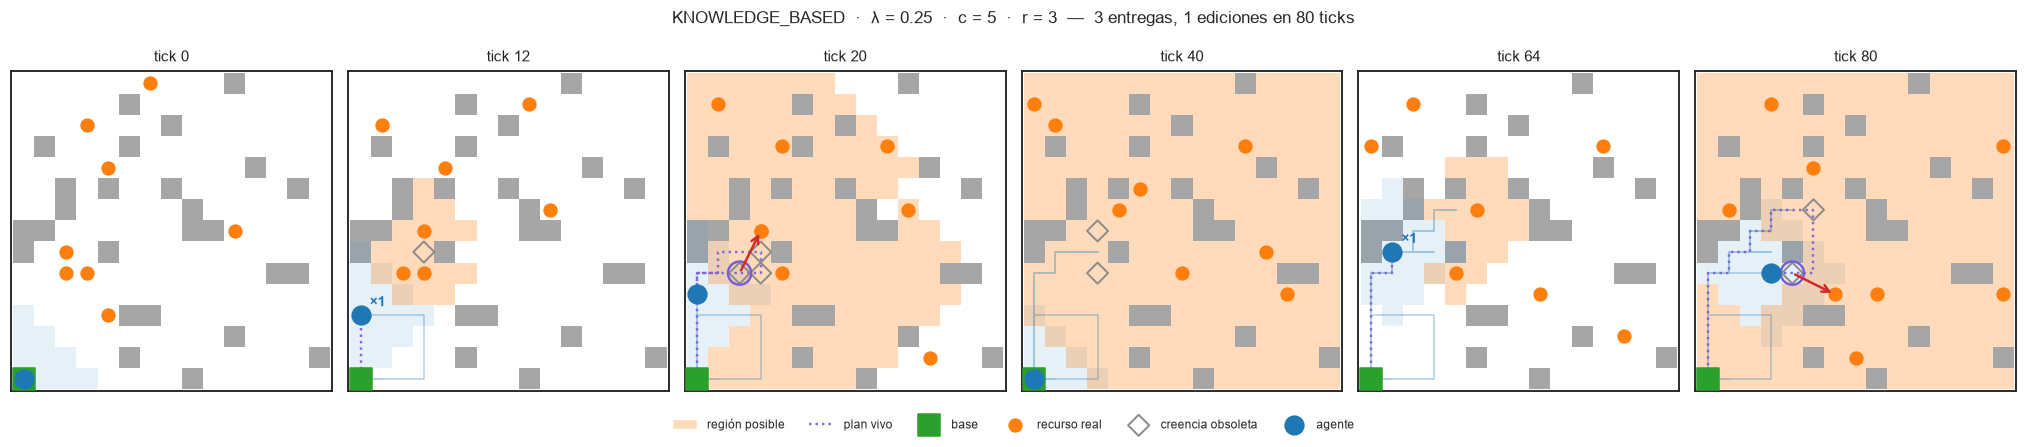
\includegraphics[width=\linewidth]{tira-knowledge-based}
  \caption{Seis instantáneas de una corrida de \KB{} ($\lambda=0.25$, $c=5$, $r=3$, semilla 3). En naranja claro, la región posible de los recursos que el agente rastrea; en naranja, la posición real de cada recurso; el rombo hueco es su última observación y la flecha roja una divergencia. En los 80 ticks el agente delibera 8 ticks, frente a 25 de \CL{} en el mismo mundo (con 3 entregas contra 4, lo cual, en una sola corrida, no dice nada sobre cuál rinde más).}
  \label{fig:tira-kb}
\end{figure}

\FloatBarrier
\subsection{El agente bayesiano}\label{sec:res-bayes}

\BY{} corre en los mismos barridos que \KB, y el cuadro~\ref{tab:bayes} reúne sus contrastes junto con el error final de su estimación de $\lambda$. HB2 pasa sin una sola corrida distinta (cuadro~\ref{tab:controles}), HB3, HB4 y HB5 se confirman, y HB1, que era la hipótesis central de esta extensión, se rechaza.

\begin{table}[htbp]
\centering
\footnotesize
\setlength{\tabcolsep}{4pt}
\begin{tabular}{@{}ll rrrr r@{}}
\toprule
$\lambda$ & $r$ & HB1: \ab{BAY}$-$\ab{KB} & \ab{BAY}$-$\ab{CL} & HB4: \ab{BAY}$-$\ab{MB} & \ab{BAY} \ahora{}$-$\ab{BAY} & Mediana $|\hat\lambda-\lambda|$ \\
\midrule
0.1  & 1        & +2.0 ± 2.6 & +3.0 ± 2.0 & \textbf{+9.7 ± 4.6} & −5.0 ± 3.1 & 0.051 \\
     & 3        & −7.0 ± 6.9 & −4.7 ± 5.7 & +12.3 ± 9.6 & +9.3 ± 6.6 & 0.021 \\
     & $\infty$ & −3.0 ± 5.3 & −3.0 ± 4.8 & \textbf{+38.0 ± 11.9} & +3.0 ± 4.8 & 0.003 \\ \sepfilas
0.25 & 1        & −3.3 ± 2.4 & −2.7 ± 3.1 & +2.0 ± 5.5 & +2.0 ± 2.6 & 0.083 \\
     & 3        & −7.7 ± 6.1 & −2.3 ± 6.0 & \textbf{−32.3 ± 9.1} & −1.0 ± 5.4 & 0.020 \\
     & $\infty$ & \textbf{−14.0 ± 5.5} & +6.0 ± 4.9 & \textbf{−51.0 ± 11.7} & −6.0 ± 4.9 & 0.005 \\ \sepfilas
0.5  & 1        & −3.0 ± 4.5 & +3.3 ± 4.2 & −8.3 ± 5.5 & −6.0 ± 4.8 & 0.080 \\
     & 3        & \textbf{−16.0 ± 4.3} & \textbf{+5.3 ± 2.4} & \textbf{−83.0 ± 10.3} & \textbf{−6.0 ± 2.6} & 0.018 \\
     & $\infty$ & −3.0 ± 2.6 & +2.0 ± 1.4 & \textbf{−117.0 ± 13.8} & −2.0 ± 1.4 & 0.005 \\
\bottomrule
\end{tabular}
\caption{Agente bayesiano ($c=5$). Las cuatro primeras columnas son diferencias pareadas de utilidad; la última, la mediana del error final de $\hat\lambda$, que sobre todo $\lambda$ vale 0.083 con $r=1$, 0.020 con $r=3$ y 0.003 con $r=\infty$.}
\label{tab:bayes}
\end{table}

\begin{itemize}[leftmargin=1.4em, itemsep=0.2em]
  \item \textbf{HB1, rechazada:} \BY{} no supera a \KB{} en ninguna celda, y queda claramente por debajo con $r=3$ y $\lambda=0.5$ (\dif{-16.0}{4.3}) y con visión total a $\lambda=0.25$ (\dif{-14.0}{5.5}), mientras que frente al lazo cerrado queda a la par en casi todo el rango.
  \item \textbf{HB3, confirmada:} La mediana de $|\hat\lambda-\lambda|$ es 0.083 con $r=1$, 0.020 con $r=3$ y 0.003 con $r=\infty$, de forma que con más visión hay más ensayos y $\lambda$ se aprende casi exacto; con $r=1$ y $\lambda=0$ el error mediano llega a 0.134, porque la previa uniforme pesa sobre pocos ensayos. La ley $1/\sqrt{n}$ en sí no se midió, porque el barrido no guarda el número de ensayos de cada corrida.
  \item \textbf{HB4, confirmada:} A $\lambda=0.5$ y $r=3$, \BY{} queda \dif{83.0}{10.3} puntos por debajo de \MB{} (15.3 contra 98.3), de modo que saber cuánto se sabe cierra 5 de los 88 puntos que separan al lazo cerrado de no planificar, menos que los 21 que cierra saber solo qué es posible.
  \item \textbf{HB5, confirmada:} El filtro está calibrado (figura~\ref{fig:fiabilidad}), pues la frecuencia observada sigue la diagonal en todo el rango, la mayor desviación en los intervalos con muchas celdas es de dos centésimas (entre 0.1 y 0.2), y los intervalos altos, con pocas celdas, tienen bandas que alcanzan la diagonal.
\end{itemize}

\begin{figure}[htbp]
  \centering
  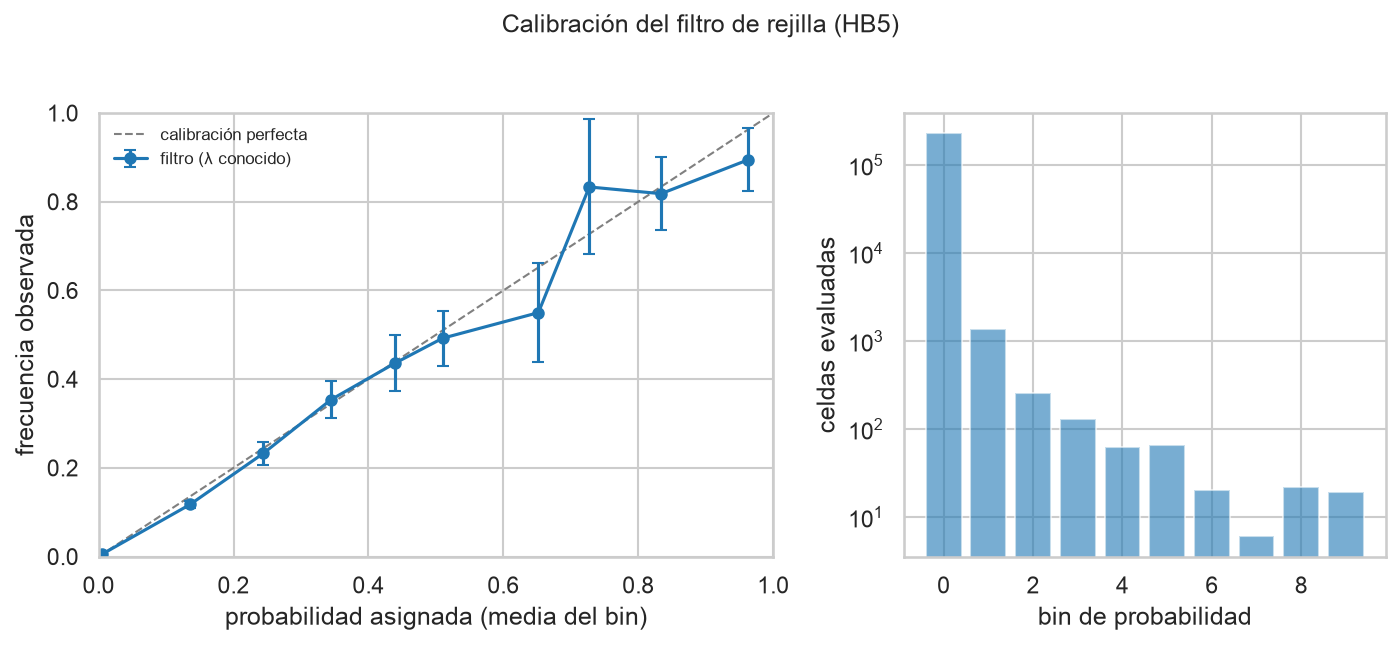
\includegraphics[width=\linewidth]{07-fiabilidad-filtro}
  \caption{Diagrama de fiabilidad del filtro de rejilla (HB5): Seis corridas cortas ($\lambda=0.25$, $r=3$, 300 ticks) en las que un filtro con $\lambda$ conocido incorpora las mismas observaciones que el agente. A la izquierda, la frecuencia con que el recurso estaba en las celdas de cada intervalo de probabilidad asignada, con su error estándar; a la derecha, el número de celdas evaluadas por intervalo, en escala logarítmica.}
  \label{fig:fiabilidad}
\end{figure}

El rechazo de HB1 no viene de la creencia sino de la decisión. Con el horizonte \ahora{} (la ablación, que deja intacta la elección de objetivo y vuelve la decisión de reparar casi idéntica al monitor del cerrado) \BY{} y \KB{} quedan ambos a la par del lazo cerrado, de modo que la diferencia entre ellos con \llegada{} está en la regla de reparación, y el cuadro~\ref{tab:mecanismo} dice en qué dirección: \BY{} repara de forma proactiva bastante más que \KB{} (6.2 contra 2.8 a $\lambda=0.1$ y 16.3 contra 9.5 a $\lambda=0.5$, cerca de las 13.7 del lazo cerrado), pasa más tiempo deliberando (265.1 contra 219.2 ticks a $\lambda=0.5$) y desperdicia más ediciones (145.8 contra 97.4). La regla $c<(1-q)(c+k)$ repara cada vez que el recurso probablemente no volverá a su celda, lo cual es correcto como predicción, pero su contabilidad de costos es incompleta en los dos lados: Por un lado, trata la reparación como si costara $c$ y comprara certeza, cuando el plan reparado nace desactualizado (el mundo sigue moviéndose durante esos $c$ ticks) y una divergencia nueva puede interrumpirlo; por otro, trata un plan mantenido que falla como si costara solo la caminata más $c$, cuando al fallar el agente suele haber perdido además de vista al objetivo, lo cual añade un costo de búsqueda que la regla no modela. La primera omisión empuja a reparar de más y es la que los datos muestran, mientras que la segunda empujaría en sentido contrario, de forma que lo prudente es concluir que, tal como está, la regla repara más de lo que conviene con dinamismo alto, y que la lógica gana justamente porque es más tacaña, pues repara solo cuando $q=0$. Cambiar de horizonte tampoco la arregla: Con \ahora, \BY{} sube de 84.3 a 93.7 a $\lambda=0.1$ (por encima de \KB{} con \llegada, 91.3, pero por debajo de su versión \ahora, 94.7, y dentro del ruido), y baja de 15.3 a 9.3 a $\lambda=0.5$ (\dif{-6.0}{2.6}).

\FloatBarrier
\subsection{Escasez: ¿vale más reparar cuando faltan recursos?}\label{sec:res-escasez}

El número de recursos estuvo fijo en 8 en todos los barridos originales, de modo que el experimento no sabía si el valor de replanificar depende de la abundancia de objetivos. La hipótesis, escrita antes de correr, era que con recursos escasos los viajes entre recogidas son más largos, el objetivo pasa más tiempo expuesto a la deriva y la reparación debería valer más. El barrido se corre en dos regímenes, uno mixto ($r=3$, $c=5$, $p=0.9$) y uno donde replanificar gana ($r=\infty$, $c=0$, $p=1$, el del control 2), y la celda con 8 recursos de cada régimen reproduce exactamente filas que ya existían (figura~\ref{fig:escasez} y cuadro~\ref{tab:escasez}).

\begin{figure}[htbp]
  \centering
  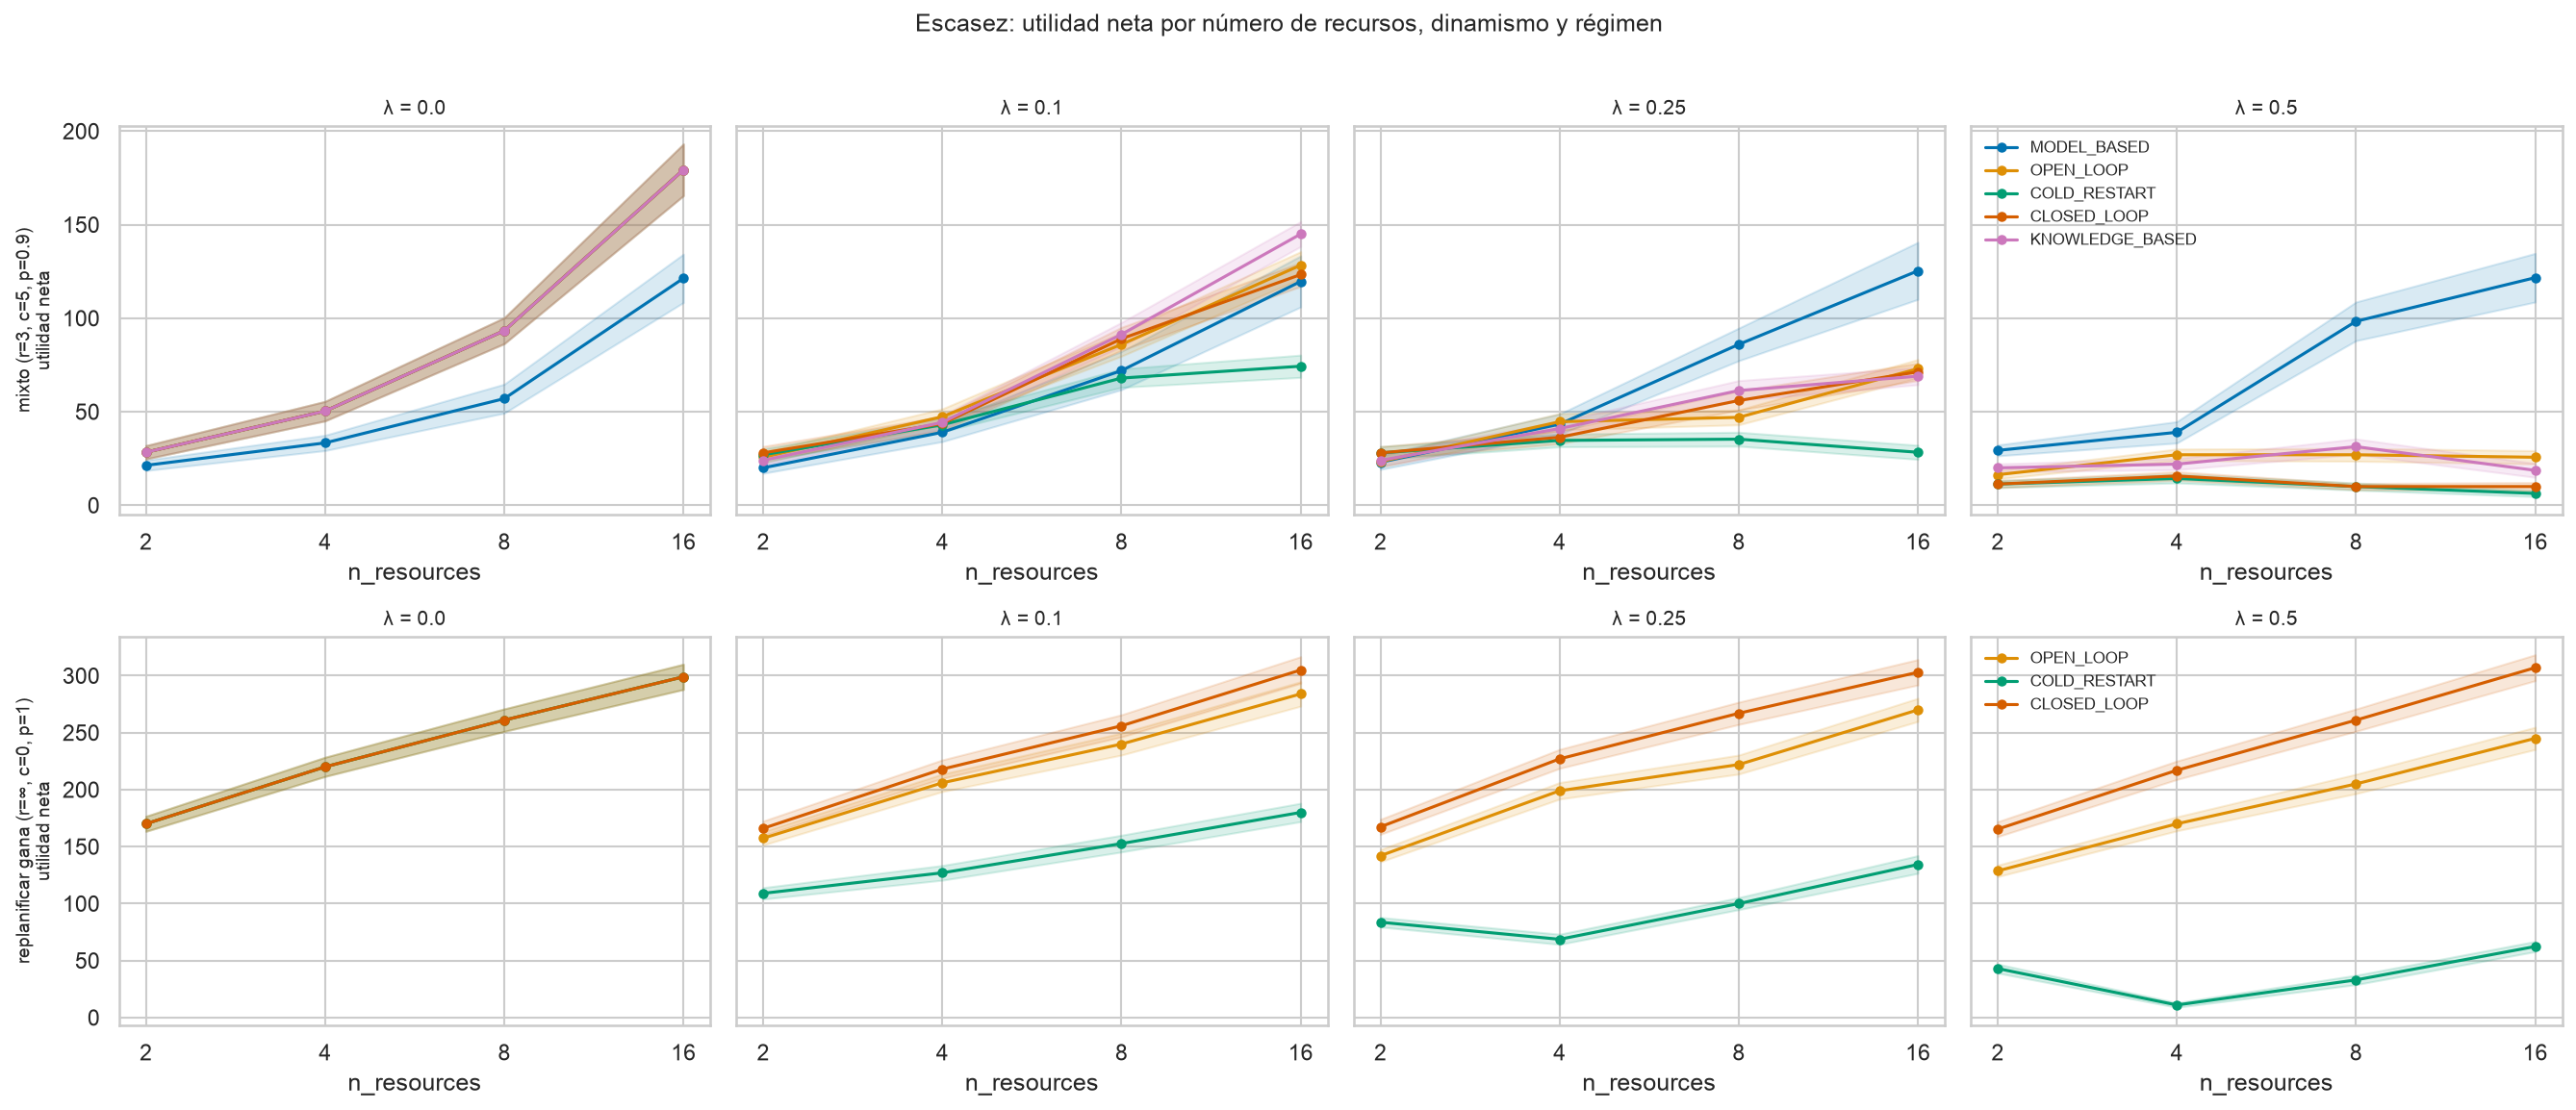
\includegraphics[width=\linewidth]{11-escasez}
  \caption{Utilidad neta por número de recursos $K$, un panel por $\lambda$. Arriba, el régimen mixto ($r=3$, $c=5$, $p=0.9$), donde con $\lambda\ge0.25$ la ventaja de \MB{} crece con la abundancia; abajo, el régimen donde replanificar gana ($r=\infty$, $c=0$, $p=1$), donde la ventaja del lazo cerrado sobre el abierto también crece con la abundancia.}
  \label{fig:escasez}
\end{figure}

\begin{table}[htbp]
\centering
\footnotesize
\begin{tabular}{@{}l l rrrr@{}}
\toprule
Contraste & $\lambda$ & $K=2$ & $K=4$ & $K=8$ & $K=16$ \\
\midrule
\multicolumn{6}{@{}l}{\emph{Régimen donde replanificar gana ($r=\infty$, $c=0$, $p=1$)}} \\
\ab{CL}$-$\ab{OL} & 0.1 & \textbf{+8.7 ± 3.5} & \textbf{+12.0 ± 4.0} & \textbf{+16.0 ± 4.5} & \textbf{+21.0 ± 4.4} \\
\ab{CL}$-$\ab{OL} & 0.5 & \textbf{+36.7 ± 4.0} & \textbf{+47.0 ± 4.0} & \textbf{+56.0 ± 4.3} & \textbf{+62.0 ± 5.0} \\
\ab{CL}$-$\ab{CR} & 0.5 & \textbf{+122.3 ± 6.0} & \textbf{+206.0 ± 7.9} & \textbf{+228.0 ± 9.7} & \textbf{+244.7 ± 10.0} \\ \sepfilas
\multicolumn{6}{@{}l}{\emph{Régimen mixto ($r=3$, $c=5$, $p=0.9$)}} \\
\ab{CL}$-$\ab{OL} & 0.25 & \textbf{+4.7 ± 1.8} & −8.3 ± 4.3 & +9.0 ± 5.7 & −1.7 ± 5.5 \\
\ab{CL}$-$\ab{OL} & 0.5 & \textbf{−5.0 ± 2.4} & \textbf{−11.3 ± 3.9} & \textbf{−17.0 ± 3.8} & \textbf{−15.7 ± 3.6} \\
\ab{CL}$-$\ab{CR} & 0.1 & +1.0 ± 1.0 & +0.7 ± 1.2 & \textbf{+21.0 ± 5.3} & \textbf{+49.0 ± 6.8} \\
\ab{CL}$-$\ab{CR} & 0.25 & 0.0 ± 0.0 & +1.7 ± 1.4 & \textbf{+20.7 ± 5.6} & \textbf{+43.0 ± 5.4} \\
\ab{MB}$-$\ab{CL} & 0.25 & −5.0 ± 3.9 & +7.0 ± 5.1 & \textbf{+30.0 ± 10.1} & \textbf{+54.0 ± 14.8} \\
\ab{MB}$-$\ab{OL} & 0.5 & \textbf{+13.0 ± 3.1} & \textbf{+12.0 ± 5.6} & \textbf{+71.3 ± 9.6} & \textbf{+96.0 ± 13.0} \\
\ab{KB}$-$\ab{CL} & 0.5 & \textbf{+8.7 ± 2.5} & +6.3 ± 3.9 & \textbf{+21.3 ± 3.8} & \textbf{+8.7 ± 3.9} \\
\bottomrule
\end{tabular}
\caption{Diferencias pareadas por número de recursos $K$ en los dos regímenes de escasez. Ninguna fila muestra que reparar valga más cuando los recursos escasean.}
\label{tab:escasez}
\end{table}

La hipótesis se refuta en los dos regímenes, pues reparar vale igual o menos con escasez, no más. Donde replanificar gana, la ventaja del lazo cerrado \emph{crece} con la abundancia, de \dif{+36.7}{4.0} sobre el abierto con 2 recursos a \dif{+62.0}{5.0} con 16 a $\lambda=0.5$, y frente al reinicio en frío de $+122.3$ a $+244.7$. En el régimen mixto el lazo cerrado no saca una ventaja consistente al abierto con $\lambda\le0.25$ en ningún número de recursos, y a $\lambda=0.5$ pierde en todos; reparar en caliente frente a en frío vale cero con 2 y 4 recursos, porque casi no hay carga a bordo que un reinicio pueda tirar (\CR{} pierde a lo sumo 0.5 unidades por corrida), y entre $+43$ y $+49$ con 16 recursos a $\lambda=0.1$ y $0.25$. Lo que sí crece con la abundancia es la ventaja de no planificar, pues a $\lambda=0.5$ la de \MB{} sobre el lazo abierto pasa de $+13.0$ con 2 recursos a $+96.0$ con 16, y a $\lambda=0.25$ su ventaja sobre el cerrado pasa de $-5.0$ a $+54.0$, es decir que la frontera entre deliberar y no deliberar se corre hacia $\lambda$ más bajos cuando sobran objetivos (con 2 y 4 recursos \MB{} solo es la mejor política a $\lambda=0.5$, y con 8 y 16, desde $\lambda=0.25$). \KB, por su parte, mantiene a $\lambda=0.5$ su ventaja sobre el lazo cerrado en toda abundancia, con el signo positivo en los cuatro niveles y fuera del ruido en tres de ellos.

La explicación es la que la hipótesis dejaba escrita para el caso contrario, el costo de oportunidad: Con objetivos escasos el cuello de botella es encontrar y alcanzar un recurso, y un tick deliberando cuesta poco porque de todos modos no había otra entrega cerca, mientras que con objetivos abundantes cada tick quieto es una entrega que se deja de hacer. El mecanismo lo muestra desde el otro lado, pues con más recursos los planes encadenan más objetivos, cada uno es una divergencia posible (a $\lambda=0.5$ el lazo cerrado pasa de 32.8 divergencias reales con 2 recursos a 78.5 con 16) y los ticks deliberando suben con ellas (de 108.6 a 309.8), justo cuando cada tick vale más, de forma que el lazo cerrado entrega lo mismo (alrededor de un recurso) con 2 que con 16 recursos, mientras que \MB{} pasa de 2.9 a 12.2 entregas. Donde deliberar es gratis no hay costo de oportunidad que pagar, y por eso en ese régimen la abundancia favorece a quien repara.

\FloatBarrier
\subsection{Sensibilidad: qué parámetro mueve qué}\label{sec:res-sensibilidad}

Sin correr nada nuevo, los cuatro barridos factoriales originales permiten preguntar qué parámetro mueve más la utilidad de cada política, con el $\eta^2$ de un factor (figura~\ref{fig:sensibilidad}), y lo mismo para la diferencia pareada \OL$-$\CL, que es la pregunta del proyecto (figura~\ref{fig:sens-delta}). Lo que ningún factor explica es interacción entre factores más la variabilidad del mundo que fija cada semilla.

\begin{figure}[htbp]
  \centering
  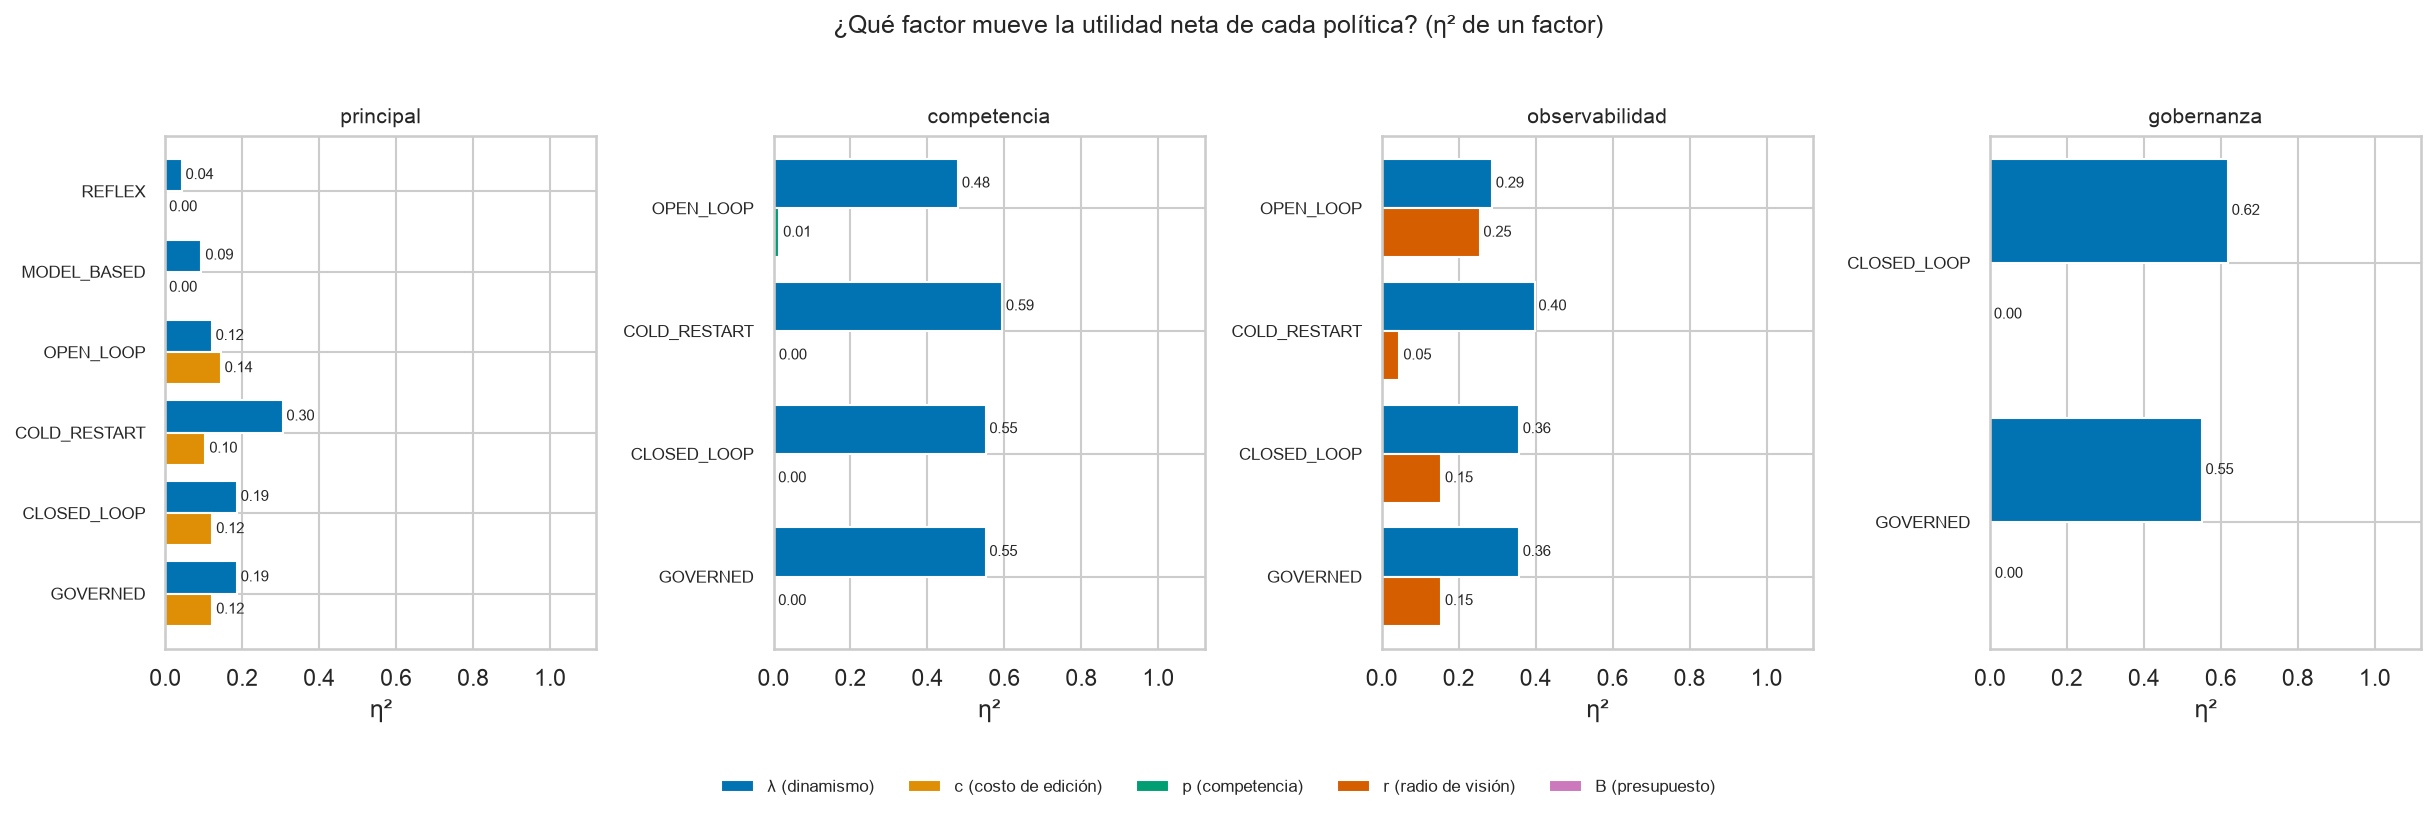
\includegraphics[width=\linewidth]{08-sensibilidad}
  \caption{Fracción de la varianza de la utilidad neta que explica cada factor barrido ($\eta^2$ de un factor), por barrido y por política. $\lambda$ domina en casi todas las políticas con plan; $p$ y $B$ no explican casi nada; \RX{} y \MB{} tienen $\eta^2=0$ para $c$, como debe ser en políticas que nunca deliberan.}
  \label{fig:sensibilidad}
\end{figure}

\begin{figure}[htbp]
  \centering
  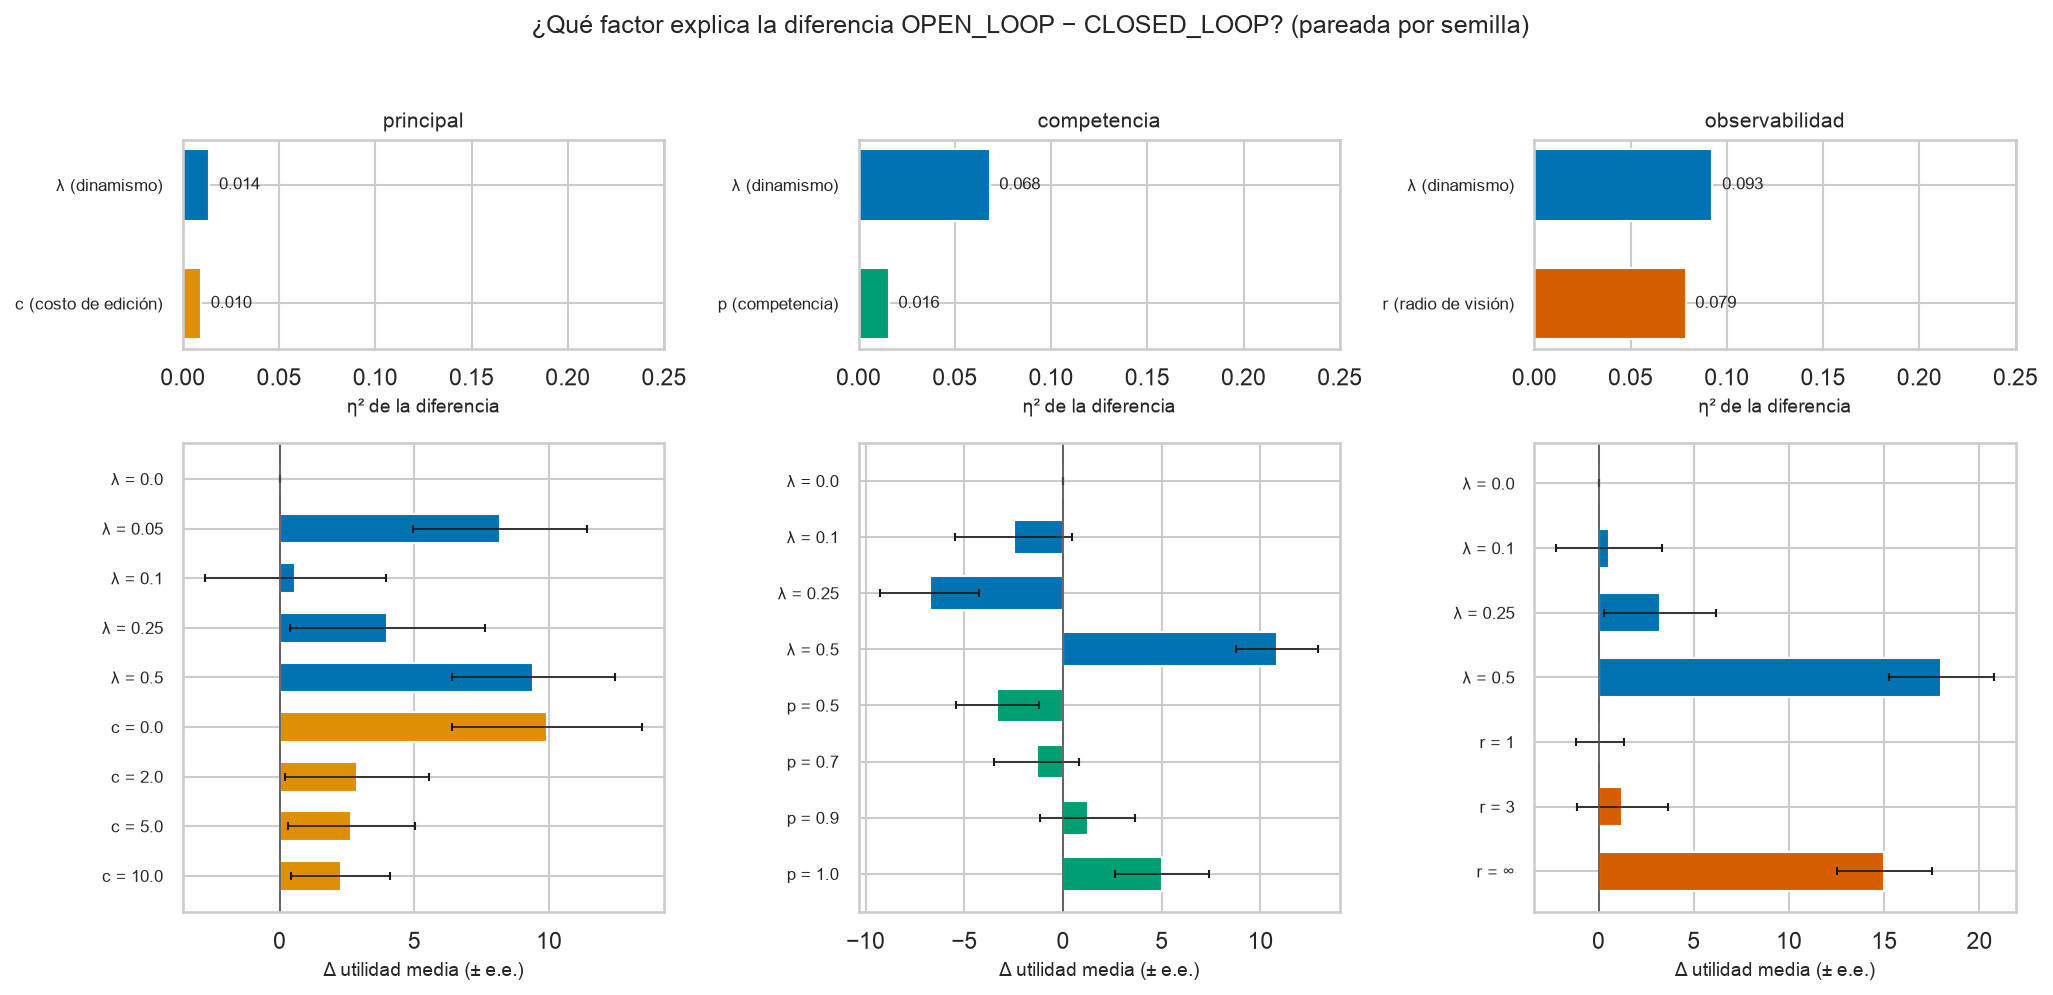
\includegraphics[width=\linewidth]{09-sensibilidad-delta}
  \caption{La misma descomposición sobre la diferencia pareada \OL$-$\CL: Arriba, el $\eta^2$ de cada factor, que no pasa de 0.093; abajo, la diferencia media ($\pm$ EE) en cada nivel, que solo se aleja de cero en los extremos ($c=0$, $\lambda=0.5$ en \texttt{competencia} y $r=\infty$).}
  \label{fig:sens-delta}
\end{figure}

Las tres hipótesis, en orden. Primeramente, $\lambda$ domina a las políticas con plan, con una excepción: En \texttt{competencia}, \texttt{observabilidad} y \texttt{gobernanza} explica entre el 29\,\% y el 62\,\% de la varianza de cada política, muy por encima de $p$ (a lo sumo 1.5\,\%), $r$ (entre 5\,\% y 25\,\%) y $B$ (a lo sumo 0.3\,\%), y en \texttt{principal} domina en \CR{} (0.305 contra 0.104 de $c$) y en \CL{} (0.186 contra 0.122), pero en \OL{} gana $c$ por poco (0.144 contra 0.121). Progresivamente, $c$ no explica más que $p$ la diferencia entre lazo abierto y cerrado, porque ninguno explica casi nada: Todos los $\eta^2$ de \OL$-$\CL{} quedan por debajo de 0.10 (en \texttt{principal}, 0.014 para $\lambda$ y 0.010 para $c$; en \texttt{competencia}, 0.068 para $\lambda$ y 0.016 para $p$), de modo que la mayor parte de su variación es ruido entre semillas y mapas, que es la contraparte estadística de la conclusión de §\ref{sec:res-frontera}; donde sí se mueve es en los extremos, con \dif{+9.9}{3.5} con $c=0$ frente a entre $+2.3$ y $+2.9$ en los otros niveles, y \dif{+15.0}{2.5} con $r=\infty$ frente a $+0.1$ y $+1.3$ con $r=1$ y $r=3$. Finalmente, $r$ mueve el nivel pero poco la diferencia solo a medias, pues explica un 25\,\% de la varianza del lazo abierto y un 15\,\% del cerrado, pero solo un 5\,\% del reinicio en frío, y sobre la diferencia explica un 8\,\%, concentrado en el salto a visión total.

Vale la pena anotar lo que dice el conjunto: En las políticas con plan, los factores barridos dejan sin explicar entre el 38\,\% (\CL{} en \texttt{gobernanza}) y el 74\,\% (\OL{} en \texttt{principal}) de la varianza, que se reparte entre interacciones ($\lambda\times c$ es justamente la frontera) y la variabilidad del mundo, por lo que comparar políticas por pares de semilla no es un lujo. Para la pregunta práctica de qué medir en un despliegue, la respuesta es $\lambda$, que es el parámetro que más mueve a toda política con plan y el que decide entre planificar y no planificar, mientras que $p$ apenas vale la pena medirlo, lo cual la calibración confirma desde otro ángulo.

\FloatBarrier
\subsection{Calibración por ABC de un despliegue}\label{sec:res-abc}

La calibración responde a la pregunta de qué haría un despliegue real con estas curvas. Un motor corre \OL{} (el modo sin monitoreo, que es lo que ejecuta un motor sin reparación en caliente) con $c=5$, $r=3$ y $(\lambda^{*}, p^{*})$ ocultos, y su telemetría da cinco tasas por tick (entregas, tareas fallidas, replanificaciones forzadas, divergencias reales y ticks deliberando), promediadas sobre cinco semillas que no pertenecen a ningún barrido. Contra la tabla de referencia (3.000 muestras de la previa uniforme $\lambda\in[0,0.8]$, $p\in[0.5,1]$), cada estadístico se estandariza por su desviación y se acepta el 5\,\% de muestras más cercano al dato (150), que aproxima la posterior. La recomendación se lee luego en dos etapas: «¿Planificar o no?» se lee de \texttt{principal}, que es el único barrido con políticas sin plan, y si la ganadora planifica, «¿abierto o cerrado?» se lee de \texttt{competencia}. Cabe mencionar que el previo de $\lambda$ llega a 0.8 a propósito, pues con el previo cortado en 0.5 el despliegue con $\lambda^{*}=0.5$ quedaba en el borde y su mediana salía en 0.39, con el precio de que para $\lambda>0.5$ la recomendación extrapola desde la última columna de los barridos.

\begin{figure}[htbp]
  \centering
  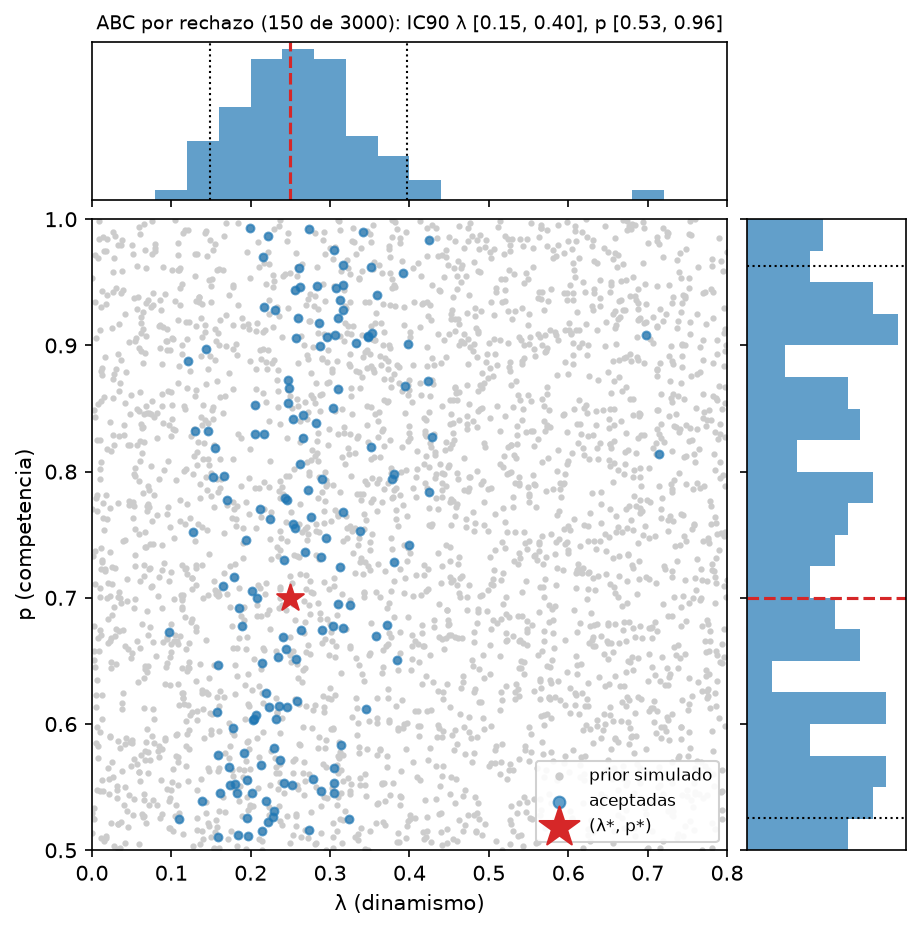
\includegraphics[width=0.62\linewidth]{10-abc}
  \caption{Posterior ABC conjunta del despliegue con $(\lambda^{*}, p^{*}) = (0.25, 0.7)$: En gris las 3.000 muestras de la previa, en azul las 150 aceptadas y la estrella en el valor verdadero; las líneas punteadas de las marginales marcan el intervalo creíble del 90\,\%. La marginal de $\lambda$ se concentra alrededor del valor verdadero, mientras que la de $p$ cubre todo el rango.}
  \label{fig:abc}
\end{figure}

\begin{table}[htbp]
\centering
\footnotesize
\begin{tabular}{@{}l l l L{5.4cm}@{}}
\toprule
$(\lambda^{*}, p^{*})$ & $\lambda$: mediana [IC 90\,\%] & $p$: mediana [IC 90\,\%] & Recomendación combinada \\
\midrule
(0.1, 0.9)  & 0.06 [0.01, 0.14] & 0.76 [0.52, 0.98] & \CL{} 81\,\%, \OL{} 15\,\%, \MB{} 3\,\% \\ \sepfilas
(0.25, 0.7) & 0.25 [0.15, 0.40] & 0.75 [0.53, 0.96] & \MB{} 87\,\%, \CL{} 8\,\%, \OL{} 5\,\% \\ \sepfilas
(0.5, 0.9)  & 0.45 [0.29, 0.74] & 0.75 [0.54, 0.95] & \MB{} 100\,\% \\
\bottomrule
\end{tabular}
\caption{Tres calibraciones de demostración con valores verdaderos conocidos. La recomendación es la fracción de la posterior en la que cada política es la mejor según la frontera barrida. Como referencia, la previa uniforme de $p$ tiene mediana 0.75 y cuantiles del 5\,\% y del 95\,\% en 0.525 y 0.975.}
\label{tab:abc}
\end{table}

La hipótesis se cumple para $\lambda$ y se queda corta para $p$ (cuadro~\ref{tab:abc} y figura~\ref{fig:abc}). Primeramente, $\lambda$ se recupera, pues el valor verdadero cae dentro del intervalo creíble del 90\,\% en los tres casos, con medianas de 0.06, 0.25 y 0.45, aunque la precisión es moderada y empeora con $\lambda$ (los intervalos miden 0.13, 0.25 y 0.45 de ancho). Progresivamente, $p$ no es identificable con esta telemetría, pues las tres posteriores son prácticamente la previa: La hipótesis esperaba una posterior ancha, pero lo que hay es ninguna información, lo cual cuadra con que $\eta^2(p)\le0.015$, ya que un parámetro que casi no mueve el resultado tampoco deja huella en la telemetría que lo resume. Finalmente, la recomendación sí es útil, pues con $\lambda^{*}=0.1$ recomienda planificar, con $\lambda^{*}=0.25$ no planificar (87\,\%) y con $\lambda^{*}=0.5$ no planificar con certeza; la decisión en dos etapas hace falta, porque leída solo en \texttt{competencia}, que no tiene políticas sin plan, la recomendación del caso intermedio sería \CL{} (79\,\%), mientras que \texttt{principal} dice que en ese dinamismo conviene no planificar (87\,\%). Vale la pena leer con cuidado el primer caso, ya que el 81\,\% de \CL{} sale de diferencias con el lazo abierto que quedan dentro del ruido a $\lambda=0.1$, de modo que lo que la calibración respalda ahí es «planificar», más que «monitorear».

\FloatBarrier
\subsection{Balance de las hipótesis}\label{sec:res-balance}

El cuadro~\ref{tab:veredictos} resume el veredicto de cada hipótesis del cuadro~\ref{tab:hipotesis}. Cabe mencionar que cuatro de ellas se rechazaron o no se sostuvieron, y que las dos arquitecturas nuevas dejan dos resultados negativos, lo cual se reporta como resultado y no como fallo del experimento.

\begin{table}[htbp]
\centering
\footnotesize
\begin{tabular}{@{}l l L{11.0cm}@{}}
\toprule
\textbf{Id.} & \textbf{Veredicto} & \textbf{Evidencia principal} \\
\midrule
O1 & Trivial & Con $\lambda=0$ empatan; con $r=3$ no hay umbral a partir del cual reparar al ver la divergencia supere a esperar el fallo (13 de 16 celdas en el ruido) \\ \sepfilas
O2 & Otra frontera & $c$ desplaza el punto desde el cual deja de convenir planificar (\MB{} gana con $\lambda=0.5$, $c\ge2$ y $\lambda=0.25$, $c\ge5$) \\ \sepfilas
O3 & No se sostiene & Control 3 solo por signo; con $p=0.5$ el cerrado supera al abierto a $\lambda=0.25$ (\dif{+11.7}{4.7}) \\ \sepfilas
O4 & En parte & $B=3$ supera a \CL{} a $\lambda=0.5$ (23.7 contra 10.0), pero $B=0$ rinde 27.0; $\eta^2(B)\le0.003$ \\ \sepfilas
O5 & Confirmada & Caliente supera a frío desde $\lambda=0.1$ ($+16$ a $+22$ con $c$ entre 2 y 5) \\ \sepfilas
Orden & Confirmada & Caliente$-$frío y \MB$-$mejor plan conservan el signo en 5 de 6 celdas; abierto$-$cerrado no tiene signo estable \\ \sepfilas
Escasez & Refutada & Reparar vale igual o menos con escasez en ambos regímenes; la explicación es el costo de oportunidad \\ \sepfilas
H1 & A medias & Signo correcto en todas las celdas; fuera del ruido solo con $r=3$, $\lambda=0.5$ (\dif{+21.3}{3.8}); desaparece en la ablación \ahora \\ \sepfilas
H1b & Solo con $\lambda=0.1$ & \dif{+5.3}{4.7} sobre \OL; \dif{-24.7}{9.8} y \dif{-67.0}{10.5} frente a \MB \\ \sepfilas
H2, HB2 & Exactas & 0 de 120 corridas distintas en cada una \\ \sepfilas
H3 & Confirmada & Un tick por consulta invierte el signo; cinco ticks cuestan hasta $-36.7$ \\ \sepfilas
H4 & Confirmada & Más fallos, menos proactivas; ahorro neto de ticks solo a $\lambda=0.5$ (\dif{-63.0}{13.6}) \\ \sepfilas
HB1 & Rechazada & \dif{-16.0}{4.3} frente a \KB{} con $r=3$, $\lambda=0.5$: La regla de utilidad esperada repara de más \\ \sepfilas
HB3 & Confirmada & Error mediano 0.083, 0.020 y 0.003 con $r=1$, 3 e $\infty$ \\ \sepfilas
HB4 & Confirmada & \dif{-83.0}{10.3} frente a \MB{} con $r=3$, $\lambda=0.5$ \\ \sepfilas
HB5 & Confirmada & Diagrama de fiabilidad sobre la diagonal \\ \sepfilas
S1 & Sí, salvo una & $\lambda$ domina salvo en \OL{} dentro de \texttt{principal} ($c$: 0.144 contra 0.121) \\ \sepfilas
S2 & No & Todos los $\eta^2$ de \OL$-$\CL{} $<0.10$: Ni $c$ ni $p$ explican casi nada \\ \sepfilas
S3 & A medias & $r$ explica 25\,\% del nivel del abierto pero 5\,\% del frío; 8\,\% de la diferencia \\ \sepfilas
ABC & A medias & $\lambda$ siempre dentro del IC 90\,\%; $p$ no identificable (posterior $\approx$ previa) \\
\bottomrule
\end{tabular}
\caption{Veredicto de las hipótesis escritas de antemano.}
\label{tab:veredictos}
\end{table}
